% Options for packages loaded elsewhere
\PassOptionsToPackage{unicode}{hyperref}
\PassOptionsToPackage{hyphens}{url}
%
\documentclass[
  man,floatsintext]{apa6}
\usepackage{amsmath,amssymb}
\usepackage{iftex}
\ifPDFTeX
  \usepackage[T1]{fontenc}
  \usepackage[utf8]{inputenc}
  \usepackage{textcomp} % provide euro and other symbols
\else % if luatex or xetex
  \usepackage{unicode-math} % this also loads fontspec
  \defaultfontfeatures{Scale=MatchLowercase}
  \defaultfontfeatures[\rmfamily]{Ligatures=TeX,Scale=1}
\fi
\usepackage{lmodern}
\ifPDFTeX\else
  % xetex/luatex font selection
\fi
% Use upquote if available, for straight quotes in verbatim environments
\IfFileExists{upquote.sty}{\usepackage{upquote}}{}
\IfFileExists{microtype.sty}{% use microtype if available
  \usepackage[]{microtype}
  \UseMicrotypeSet[protrusion]{basicmath} % disable protrusion for tt fonts
}{}
\makeatletter
\@ifundefined{KOMAClassName}{% if non-KOMA class
  \IfFileExists{parskip.sty}{%
    \usepackage{parskip}
  }{% else
    \setlength{\parindent}{0pt}
    \setlength{\parskip}{6pt plus 2pt minus 1pt}}
}{% if KOMA class
  \KOMAoptions{parskip=half}}
\makeatother
\usepackage{xcolor}
\usepackage{color}
\usepackage{fancyvrb}
\newcommand{\VerbBar}{|}
\newcommand{\VERB}{\Verb[commandchars=\\\{\}]}
\DefineVerbatimEnvironment{Highlighting}{Verbatim}{commandchars=\\\{\}}
% Add ',fontsize=\small' for more characters per line
\usepackage{framed}
\definecolor{shadecolor}{RGB}{248,248,248}
\newenvironment{Shaded}{\begin{snugshade}}{\end{snugshade}}
\newcommand{\AlertTok}[1]{\textcolor[rgb]{0.94,0.16,0.16}{#1}}
\newcommand{\AnnotationTok}[1]{\textcolor[rgb]{0.56,0.35,0.01}{\textbf{\textit{#1}}}}
\newcommand{\AttributeTok}[1]{\textcolor[rgb]{0.13,0.29,0.53}{#1}}
\newcommand{\BaseNTok}[1]{\textcolor[rgb]{0.00,0.00,0.81}{#1}}
\newcommand{\BuiltInTok}[1]{#1}
\newcommand{\CharTok}[1]{\textcolor[rgb]{0.31,0.60,0.02}{#1}}
\newcommand{\CommentTok}[1]{\textcolor[rgb]{0.56,0.35,0.01}{\textit{#1}}}
\newcommand{\CommentVarTok}[1]{\textcolor[rgb]{0.56,0.35,0.01}{\textbf{\textit{#1}}}}
\newcommand{\ConstantTok}[1]{\textcolor[rgb]{0.56,0.35,0.01}{#1}}
\newcommand{\ControlFlowTok}[1]{\textcolor[rgb]{0.13,0.29,0.53}{\textbf{#1}}}
\newcommand{\DataTypeTok}[1]{\textcolor[rgb]{0.13,0.29,0.53}{#1}}
\newcommand{\DecValTok}[1]{\textcolor[rgb]{0.00,0.00,0.81}{#1}}
\newcommand{\DocumentationTok}[1]{\textcolor[rgb]{0.56,0.35,0.01}{\textbf{\textit{#1}}}}
\newcommand{\ErrorTok}[1]{\textcolor[rgb]{0.64,0.00,0.00}{\textbf{#1}}}
\newcommand{\ExtensionTok}[1]{#1}
\newcommand{\FloatTok}[1]{\textcolor[rgb]{0.00,0.00,0.81}{#1}}
\newcommand{\FunctionTok}[1]{\textcolor[rgb]{0.13,0.29,0.53}{\textbf{#1}}}
\newcommand{\ImportTok}[1]{#1}
\newcommand{\InformationTok}[1]{\textcolor[rgb]{0.56,0.35,0.01}{\textbf{\textit{#1}}}}
\newcommand{\KeywordTok}[1]{\textcolor[rgb]{0.13,0.29,0.53}{\textbf{#1}}}
\newcommand{\NormalTok}[1]{#1}
\newcommand{\OperatorTok}[1]{\textcolor[rgb]{0.81,0.36,0.00}{\textbf{#1}}}
\newcommand{\OtherTok}[1]{\textcolor[rgb]{0.56,0.35,0.01}{#1}}
\newcommand{\PreprocessorTok}[1]{\textcolor[rgb]{0.56,0.35,0.01}{\textit{#1}}}
\newcommand{\RegionMarkerTok}[1]{#1}
\newcommand{\SpecialCharTok}[1]{\textcolor[rgb]{0.81,0.36,0.00}{\textbf{#1}}}
\newcommand{\SpecialStringTok}[1]{\textcolor[rgb]{0.31,0.60,0.02}{#1}}
\newcommand{\StringTok}[1]{\textcolor[rgb]{0.31,0.60,0.02}{#1}}
\newcommand{\VariableTok}[1]{\textcolor[rgb]{0.00,0.00,0.00}{#1}}
\newcommand{\VerbatimStringTok}[1]{\textcolor[rgb]{0.31,0.60,0.02}{#1}}
\newcommand{\WarningTok}[1]{\textcolor[rgb]{0.56,0.35,0.01}{\textbf{\textit{#1}}}}
\usepackage{graphicx}
\makeatletter
\def\maxwidth{\ifdim\Gin@nat@width>\linewidth\linewidth\else\Gin@nat@width\fi}
\def\maxheight{\ifdim\Gin@nat@height>\textheight\textheight\else\Gin@nat@height\fi}
\makeatother
% Scale images if necessary, so that they will not overflow the page
% margins by default, and it is still possible to overwrite the defaults
% using explicit options in \includegraphics[width, height, ...]{}
\setkeys{Gin}{width=\maxwidth,height=\maxheight,keepaspectratio}
% Set default figure placement to htbp
\makeatletter
\def\fps@figure{htbp}
\makeatother
\setlength{\emergencystretch}{3em} % prevent overfull lines
\providecommand{\tightlist}{%
  \setlength{\itemsep}{0pt}\setlength{\parskip}{0pt}}
\setcounter{secnumdepth}{-\maxdimen} % remove section numbering
% Make \paragraph and \subparagraph free-standing
\ifx\paragraph\undefined\else
  \let\oldparagraph\paragraph
  \renewcommand{\paragraph}[1]{\oldparagraph{#1}\mbox{}}
\fi
\ifx\subparagraph\undefined\else
  \let\oldsubparagraph\subparagraph
  \renewcommand{\subparagraph}[1]{\oldsubparagraph{#1}\mbox{}}
\fi
\newlength{\cslhangindent}
\setlength{\cslhangindent}{1.5em}
\newlength{\csllabelwidth}
\setlength{\csllabelwidth}{3em}
\newlength{\cslentryspacingunit} % times entry-spacing
\setlength{\cslentryspacingunit}{\parskip}
\newenvironment{CSLReferences}[2] % #1 hanging-ident, #2 entry spacing
 {% don't indent paragraphs
  \setlength{\parindent}{0pt}
  % turn on hanging indent if param 1 is 1
  \ifodd #1
  \let\oldpar\par
  \def\par{\hangindent=\cslhangindent\oldpar}
  \fi
  % set entry spacing
  \setlength{\parskip}{#2\cslentryspacingunit}
 }%
 {}
\usepackage{calc}
\newcommand{\CSLBlock}[1]{#1\hfill\break}
\newcommand{\CSLLeftMargin}[1]{\parbox[t]{\csllabelwidth}{#1}}
\newcommand{\CSLRightInline}[1]{\parbox[t]{\linewidth - \csllabelwidth}{#1}\break}
\newcommand{\CSLIndent}[1]{\hspace{\cslhangindent}#1}
\ifLuaTeX
\usepackage[bidi=basic]{babel}
\else
\usepackage[bidi=default]{babel}
\fi
\babelprovide[main,import]{english}
% get rid of language-specific shorthands (see #6817):
\let\LanguageShortHands\languageshorthands
\def\languageshorthands#1{}
% Manuscript styling
\usepackage{upgreek}
\captionsetup{font=singlespacing,justification=justified}

% Table formatting
\usepackage{longtable}
\usepackage{lscape}
% \usepackage[counterclockwise]{rotating}   % Landscape page setup for large tables
\usepackage{multirow}		% Table styling
\usepackage{tabularx}		% Control Column width
\usepackage[flushleft]{threeparttable}	% Allows for three part tables with a specified notes section
\usepackage{threeparttablex}            % Lets threeparttable work with longtable

% Create new environments so endfloat can handle them
% \newenvironment{ltable}
%   {\begin{landscape}\centering\begin{threeparttable}}
%   {\end{threeparttable}\end{landscape}}
\newenvironment{lltable}{\begin{landscape}\centering\begin{ThreePartTable}}{\end{ThreePartTable}\end{landscape}}

% Enables adjusting longtable caption width to table width
% Solution found at http://golatex.de/longtable-mit-caption-so-breit-wie-die-tabelle-t15767.html
\makeatletter
\newcommand\LastLTentrywidth{1em}
\newlength\longtablewidth
\setlength{\longtablewidth}{1in}
\newcommand{\getlongtablewidth}{\begingroup \ifcsname LT@\roman{LT@tables}\endcsname \global\longtablewidth=0pt \renewcommand{\LT@entry}[2]{\global\advance\longtablewidth by ##2\relax\gdef\LastLTentrywidth{##2}}\@nameuse{LT@\roman{LT@tables}} \fi \endgroup}

% \setlength{\parindent}{0.5in}
% \setlength{\parskip}{0pt plus 0pt minus 0pt}

% Overwrite redefinition of paragraph and subparagraph by the default LaTeX template
% See https://github.com/crsh/papaja/issues/292
\makeatletter
\renewcommand{\paragraph}{\@startsection{paragraph}{4}{\parindent}%
  {0\baselineskip \@plus 0.2ex \@minus 0.2ex}%
  {-1em}%
  {\normalfont\normalsize\bfseries\itshape\typesectitle}}

\renewcommand{\subparagraph}[1]{\@startsection{subparagraph}{5}{1em}%
  {0\baselineskip \@plus 0.2ex \@minus 0.2ex}%
  {-\z@\relax}%
  {\normalfont\normalsize\itshape\hspace{\parindent}{#1}\textit{\addperi}}{\relax}}
\makeatother

\makeatletter
\usepackage{etoolbox}
\patchcmd{\maketitle}
  {\section{\normalfont\normalsize\abstractname}}
  {\section*{\normalfont\normalsize\abstractname}}
  {}{\typeout{Failed to patch abstract.}}
\patchcmd{\maketitle}
  {\section{\protect\normalfont{\@title}}}
  {\section*{\protect\normalfont{\@title}}}
  {}{\typeout{Failed to patch title.}}
\makeatother

\usepackage{xpatch}
\makeatletter
\xapptocmd\appendix
  {\xapptocmd\section
    {\addcontentsline{toc}{section}{\appendixname\ifoneappendix\else~\theappendix\fi\\: #1}}
    {}{\InnerPatchFailed}%
  }
{}{\PatchFailed}
\keywords{Educational Outcomes, School Quality, Education}
\DeclareDelayedFloatFlavor{ThreePartTable}{table}
\DeclareDelayedFloatFlavor{lltable}{table}
\DeclareDelayedFloatFlavor*{longtable}{table}
\makeatletter
\renewcommand{\efloat@iwrite}[1]{\immediate\expandafter\protected@write\csname efloat@post#1\endcsname{}}
\makeatother
\usepackage{csquotes}
\ifLuaTeX
  \usepackage{selnolig}  % disable illegal ligatures
\fi
\IfFileExists{bookmark.sty}{\usepackage{bookmark}}{\usepackage{hyperref}}
\IfFileExists{xurl.sty}{\usepackage{xurl}}{} % add URL line breaks if available
\urlstyle{same}
\hypersetup{
  pdftitle={An Analysis of the Department of Education Quality Survey and Its Efficacy},
  pdfauthor={Andrew Bowen1, Glen Dale Davis1, Josh Forster1, Shoshana Farber1, \& Charles Ugiagbe1},
  pdflang={en-EN},
  pdfkeywords={Educational Outcomes, School Quality, Education},
  hidelinks,
  pdfcreator={LaTeX via pandoc}}

\title{An Analysis of the Department of Education Quality Survey and Its Efficacy}
\author{Andrew Bowen\textsuperscript{1}, Glen Dale Davis\textsuperscript{1}, Josh Forster\textsuperscript{1}, Shoshana Farber\textsuperscript{1}, \& Charles Ugiagbe\textsuperscript{1}}
\date{}


\shorttitle{DATA621 Final Project}

\affiliation{\vspace{0.5cm}\textsuperscript{1} City University of New York}

\abstract{%
We present a study on the effectiveness of New York City School Quality Snapshot in predicting the 4-year college persistence rate for New York City high schools. These surveys are used in the deciding of educational policy across the United States. While input from educators and families can be invaluable, it often can not reflect the underlying factors that most influence academic performance. We also build a predictive model based on proxy socioeconomic factors (presence in temporary housing, economic need) that can also be used to predict the average college persistence of a high school in NYC. Our model based on socioeconomic indicators outperforms a model based solely on results of the school quality snapshot, which includes survey responses from students, parents, and educators within NYC public schools. This increased performance comes across several model diagnostic statistics, including root mean-squared error, Akaike and Bayesian Information Criteria, and adjusted R-squared. Additionally, a weighted least-squares model is created on the same set of proxy variables to compare modeling techniques. This model outperforms the ratings-based linear model, but introduces additional complexity for less explainability when compared with the direct proxy variable model.
}



\begin{document}
\maketitle

\hypertarget{introduction}{%
\section{Introduction}\label{introduction}}

The NYC School Survey seeks to collect data to provide an overview of New York City (NYC) Schools. First conducted in 2005, the survey gathers demographic and achievement data for NYC Public Schools and provides a standardized rating of various elements of school quality.

The survey has changed over the years. These changes have come from the recommendations of public policy analysts seeking to more accurately define the quality of schools \emph{New York City Schools (2018)}. The 2020-21 academic year report provides a robust dataset of school-level observations of academic and socioeconomic data.

\textbf{Research Question:} Our analysis aims to determine whether NYC School Quality Survey ratings accurately reflect educational outcomes or if these outcomes could be better predicted by proxy variables related to the student body.

The primary measure of success we aim to predict is the 4-year college persistence rate for NYC high schools. This measure is defined as the percentage of students who graduate from a high school and eventually complete a 4-year college program. Identifying the key indicators of a school's ability to successfully prepare students for college could benefit the NYC Department of Education (DOE) and NYC Public Schools in several ways:

\begin{enumerate}
\def\labelenumi{\arabic{enumi}.}
\tightlist
\item
  It would provide insights to the NYC DOE and NYC Public Schools which would enable them to tailor instructional approaches and develop targeted curricula that specifically address college preparedness.
\item
  It would allow for strategic allocation of resources to address identified areas that significantly impact college readiness, ensuring that resources are utilized efficiently to increase the percentage of college-ready students across NYC Public Schools.
\end{enumerate}

It is well-established that attending 4-year institutions significantly enhances career potential earnings. Ensuring that high school students are adequately prepared for their college careers not only benefits their immediate educational success but also contributes to their long-term success in life.

\hypertarget{literature-review}{%
\section{Literature Review}\label{literature-review}}

One of the main predictors of academic performance is a student's socioeconomic background. According to the National Center for Education Statistics (NCES), students from low-income families are nearly four times more likely to drop out of high school than students from wealthy families \emph{Education Statistics (2008)}.

Several prior studies have made attempts to use more sophisticated modeling techniques, different data sources, and different predictor variables to predict educational outcomes similar to what we're trying to predict. In one such study, \emph{Bernacki, Chavez, and Uesbeck (2020)} based their modeling on trying to predict educational achievement based on student digital behavior, rather than the social factors we intend to explore. The model in this study reached an accuracy of 75\%, and was able to flag early interventions. This modeling technique attempts to predict a slightly different metric of student success than our modeling will, and the training data and predictor variables differ as well.

Similarly, \emph{Musso, Cascallar, Bostani, and Crawford (2020)} attempted to train an artificial neural network (ANN) to identify relationships between variables and educational performance data. They modeled educational performance of Vietnamese students in grade five and included individual characteristics as well as information related to daily routines in their training data. This method uses a more sophisticated model, and resulted in an impressive prediction accuracy of \(95-100%
\). However, as their training data comes from a different country with a different educational system and methods, it may not be prudent to compare the model's results to those of our model or of any other US-centric study.

In another study, \emph{Yağcı (2022)} predicted final grade exams for Turkish students through machine learning models, using prior exam scores as their input variables. While this provides a valuable metric for academic performance, concerns arise regarding the direct correlation between good exam grades and later career success \emph{Afarian and Kleiner (2003)}. However, a parent study found a correlation of up to 0.3 between academic grades and later job performance \emph{Roth, BeVier, Switzer III, and Schippmann (1996)}, so it may be worthwhile to consider this metric as a measure to predict later success in life. Further analysis would have to be conducted in this respect.

Measuring which predictors impact educational outcomes and how much is a difficult task. There are generally many confounding variables related to the student body being observed, and causal relationships can be difficult if not impossible to establish.

\hypertarget{data-sourcing}{%
\section{Data Sourcing}\label{data-sourcing}}

The dataset used in this study is published in the \href{https://data.cityofnewyork.us/Education/2020-2021-School-Quality-Reports-High-School/26je-vkp6}{NYC School Quality Report for the Academic Year 2020 - 2021}. It consists of data from 487 NYC Public Schools, and there are 391 variable columns. The observations are all school-level, indexed by each school's \emph{District Borough Number} (DBN).

In addition to the school quality ratings based on survey responses, average and raw academic performance data are included as well. There are also socioeconomic variables, such as a school's percentage of students in temporary housing services.

\hypertarget{methodology}{%
\section{Methodology}\label{methodology}}

Our primary interest is finding proxy variables within the data that can better serve as predictors of 4-year college persistence rates at a given NYC high school than the school survey ratings collected by the quality review. Toward this end, we will need to first construct a baseline model that predicts a school's college persistence rate.

We will attempt to use three variables as a proxy for the school's survey rating in predicting college persistence:

\begin{itemize}
\tightlist
\item
  \texttt{temp\_housing\_pct}: the percentage of students living in temporary housing
\item
  \texttt{eni\_hs\_pct\_912}: \href{https://data.cccnewyork.org/data/bar/1371/student-economic-need-index\#1371/a/1/1622/127}{Economic Need Index}: a measure of the percentage of students facing economic hardship at a school\footnote{\textbf{noauthor\_student\_2021 (fix, not in references)} Economic hardship in this context is based on three criteria: whether the student is 1) eligible for public assistance from the NYC Human Resources Administration (HRA); 2) lived in temporary housing in the past four years; 3) is in high school, has a home language other than English, and entered the NYC DOE for the first time within the last four years.}
\item
  \texttt{val\_chronic\_absent\_hs\_all}: the percentage of students who are chronically absent\footnote{Chronic absenteeism is defined by the NYC DOE as ``students who are absent 10 percent or more of the total days.''}
\end{itemize}

We begin by taking a look at a summary of the dataset's completeness.

\begin{table}[H]

\begin{center}
\begin{threeparttable}

\caption{\label{tab:data2}Completeness Summary}

\begin{tabular}{ll}
\toprule
 & \multicolumn{1}{c}{}\\
\midrule
rows & 487\\
columns & 393\\
all\_missing\_columns & 12\\
total\_missing\_values & 47359\\
complete\_rows & 0\\
\bottomrule
\end{tabular}

\end{threeparttable}
\end{center}

\end{table}

There are 12 columns that are completely devoid of data, so we identify and remove those.

\begin{table}[H]

\begin{center}
\begin{threeparttable}

\caption{\label{tab:unnamed-chunk-2}}

\begin{tabular}{l}
\toprule
All NA Columns\\
\midrule
QR\_1\_1\\
QR\_1\_2\\
QR\_2\_2\\
QR\_3\_4\\
QR\_4\_2\\
QR\_1\_4\\
QR\_1\_3\\
QR\_3\_1\\
QR\_4\_1\\
QR\_5\_1\\
Dates\_of\_Review\\
principal\\
\bottomrule
\end{tabular}

\end{threeparttable}
\end{center}

\end{table}

We create a 20\% holdout set of data to be used later on in order to evaluate the efficacy of our model's predictive capability. The remaining 80\% of the data is to be used for model training and exploratory data analysis (EDA).

For ease of single-node computation, we'll select the variables of interest from our dataset. Notably, these are the survey ratings, enrollment levels, and our preferred proxy variables for each school.

We take a look at whether the reduced training dataset contains any missing values and what the spread is.

\begin{figure}[H]
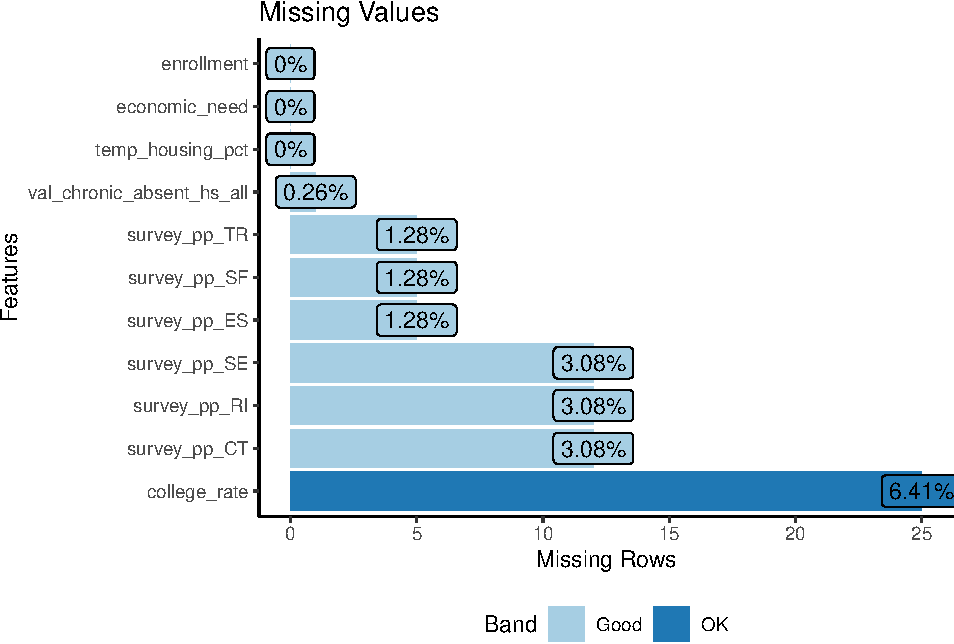
\includegraphics[width=\textwidth]{final-project_files/figure-latex/data4-1} \caption{ }\label{fig:data4}
\end{figure}

The variable with the most missing data is \texttt{college\_rate}. Some schools are also missing some survey ratings, and a very small percentage of schools are missing chronic absenteeism values.

We impute both our training and evaluation datasets. Given we are dealing with continuous numeric (and not categorical variables), we use the \emph{Predictive Mean Matching} imputation method native to the R \texttt{mice} package.

To check underlying modeling assumptions, we plot distributions and relationships of different variables. First, we plot the distribution of college persistence rates among NYC high schools to check for normality.

\begin{figure}[H]
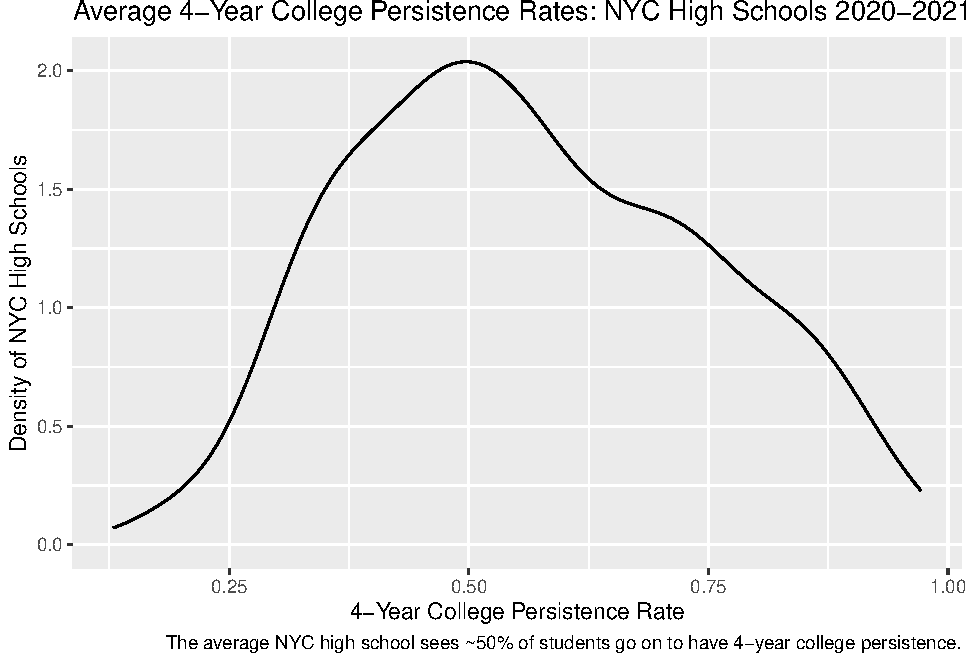
\includegraphics[width=\textwidth]{final-project_files/figure-latex/unnamed-chunk-4-1} \caption{ }\label{fig:unnamed-chunk-4}
\end{figure}

We see a relatively normal distribution of college persistence rates. In the case of NYC high schools, the peak is at around 50\%. This is inline with national averages released by the \emph{US Census Bureau (2023)}.

The below plot shows the raw correlation between each variable in our pared down dataset (\emph{Collaborative Teaching}, \emph{Trust}, etc) and the response variable of interest: \emph{4-Year College Persistence Rate}.

\begin{figure}[H]
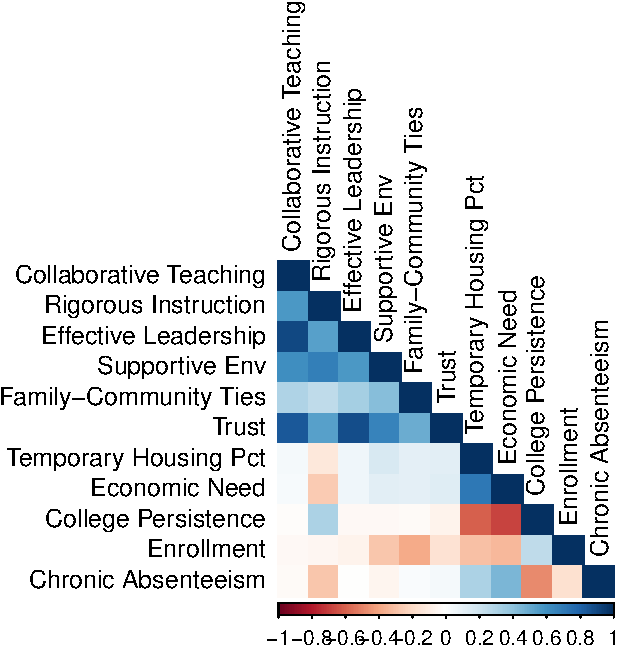
\includegraphics[width=\textwidth]{final-project_files/figure-latex/unnamed-chunk-5-1} \caption{ }\label{fig:unnamed-chunk-5}
\end{figure}

From our correlation plot above, we can see strong negative relationships between two of our proxy variables of interest (\emph{Temporary Housing Rate} and \emph{Economic Need Index}) and our target variable: \emph{College Persistence Rate}. There is also a negative relationship between \emph{Chronic Absenteeism} and \emph{College Persistence Rate}, but to a lesser degree. This gives signal that constructing models based on these variables could give good insight into the factors that most influence college persistence.

\emph{Enrollment} has only a slightly positive relationship with \emph{College Persistence Rate}. We expected school size might be important when modeling, but that does not appear to be likely.

We also see that the survey ratings are all at least somewhat positively correlated with one another, and the only survey rating that appears to have a relationship with \emph{College Persistence Rate} is \emph{Rigorous Instruction}. That relationship is only slightly positive. This signals that constructing a model based on one or more of the survey ratings might not give as much insight into college persistence as the proxy variables could.

Now we can plot the distributions of our proxy variables of interest.

\begin{figure}[H]
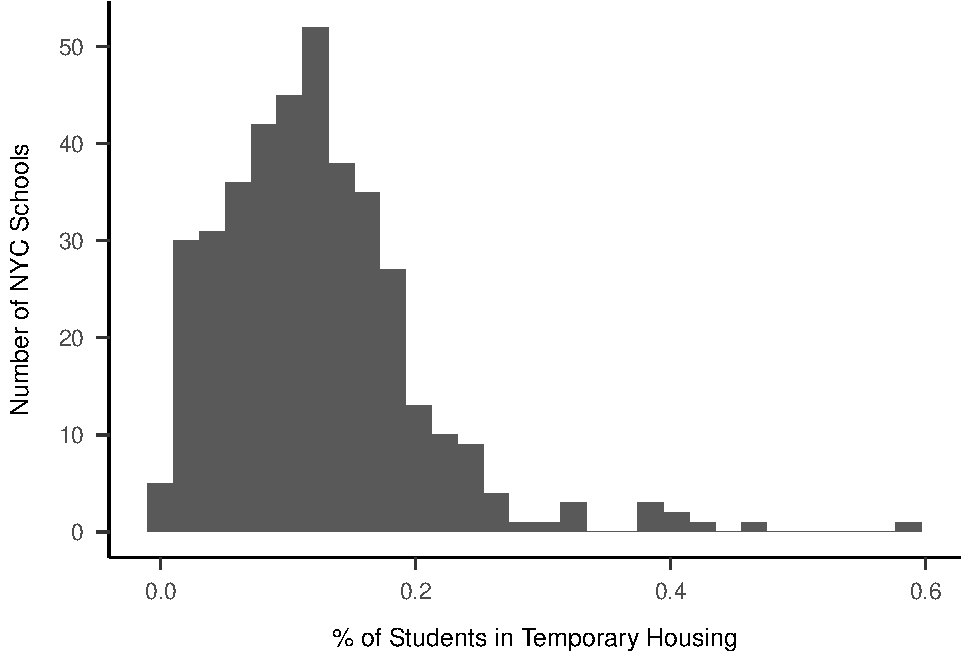
\includegraphics[width=\textwidth]{final-project_files/figure-latex/temp-housing-rates-1} \caption{ }\label{fig:temp-housing-rates}
\end{figure}

We see the distribution of \emph{Temporary Housing Rate} is right-skewed. We also see the distribution of \emph{Economic Need Index} is left-skewed. The closer the index is to 1, the more economic hardship students at that school face, so schools with high rates of students facing economic hardship are more prevalent than schools with low rates. These variables are both candidates for transformation due to their skew. Our model will not likely feature \emph{Enrollment}, as observations are so concentrated at the low end, and we already noted it is not as correlated with our target variable as the other proxies we're considering. \emph{Chronic Absenteeism} is closer to a normal distribution than the other variables, but it is still slightly right-skewed, so there are more schools in this dataset with pretty low rates and fewer schools with pretty high rates.

We check an assumption of linearity between our proxy predictors and our response variable by producing scatter plots of the response variable versus each of the proxy predictors.

\begin{figure}[H]
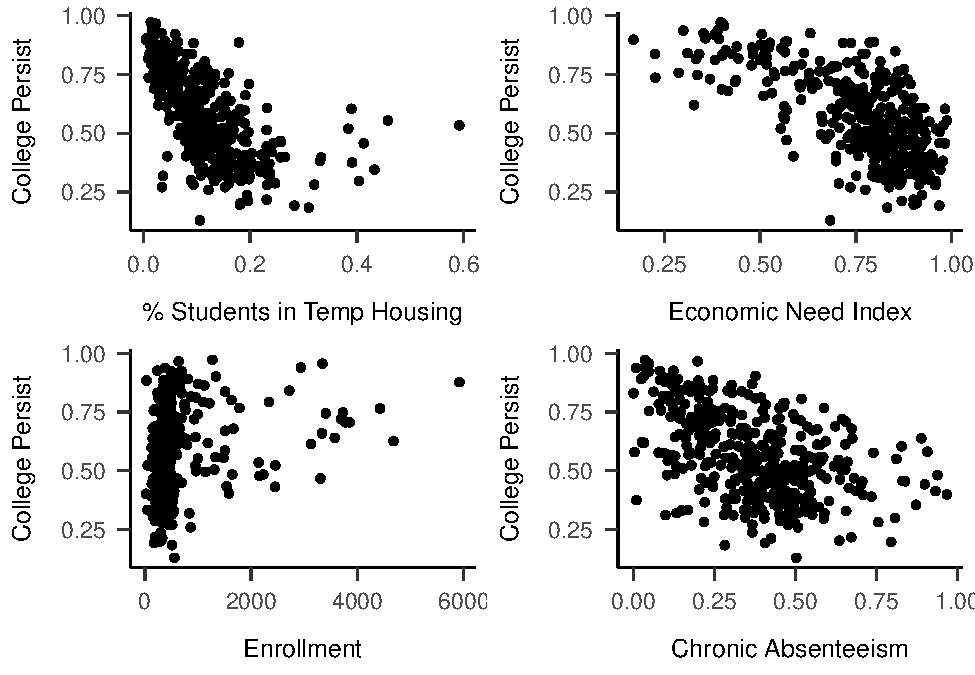
\includegraphics[width=\textwidth]{final-project_files/figure-latex/unnamed-chunk-6-1} \caption{ }\label{fig:unnamed-chunk-6}
\end{figure}

We see a generally negative linear relationship between the response variable and rates of students in temporary housing. As that rate increases, college persistence tends to decrease. However, that relationship does \textbf{not} appear to hold for schools with higher rates of students in temporary housing. So the relationship cannot be completely captured by a linear trend.

We also see a non-linear relationship between the response variable and the economic need index.

Schools with lower enrollment levels have a wider range of college persistence rates than schools with higher enrollment levels.

Only one school where chronic absenteeism is greater than or equal to 50 percent achieves college persistence levels above 80 percent. However, college persistence varies widely at most chronic absenteeism levels.

\hypertarget{modeling}{%
\section{Modeling}\label{modeling}}

For evaluation purposes, we create a linear model based on the survey ratings present per school in our data. We fit this multiple least-squares model to predict the college persistence rate of a given high school. The model summary is printed below:

\begin{verbatim}
## 
## Call:
## lm(formula = base_formula, data = train)
## 
## Residuals:
##     Min      1Q  Median      3Q     Max 
## -0.5405 -0.1119  0.0053  0.1135  0.4303 
## 
## Coefficients:
##              Estimate Std. Error t value Pr(>|t|)    
## (Intercept)    0.5399     0.1976   2.732  0.00659 ** 
## survey_pp_CT   0.1150     0.2635   0.436  0.66281    
## survey_pp_RI   2.1733     0.1976  11.001  < 2e-16 ***
## survey_pp_SE  -1.5105     0.2664  -5.671  2.8e-08 ***
## survey_pp_ES  -0.3090     0.2802  -1.103  0.27079    
## survey_pp_SF   0.2349     0.2131   1.102  0.27109    
## survey_pp_TR  -0.4708     0.4237  -1.111  0.26724    
## ---
## Signif. codes:  0 '***' 0.001 '**' 0.01 '*' 0.05 '.' 0.1 ' ' 1
## 
## Residual standard error: 0.1581 on 383 degrees of freedom
## Multiple R-squared:  0.2495, Adjusted R-squared:  0.2377 
## F-statistic: 21.22 on 6 and 383 DF,  p-value: < 2.2e-16
\end{verbatim}

We find our base model for the school survey ratings produces an adjusted R-squared of \(R^2_{adj} = 0.24\). This is lower than the predictive model in \emph{Roth et al. (1996)} produces. The two survey ratings that appear to be statistically significant to the model are \emph{Rigorous Instruction}, which we expected based on our correlation analysis, and \emph{Supportive Environment}, which we did not expect. We reduce the model via backward selection, and \emph{Effective Leadership} becomes statistically significant as well. We reprint a summary below:

\begin{verbatim}
## 
## Call:
## lm(formula = college_rate ~ survey_pp_RI + survey_pp_SE + survey_pp_ES, 
##     data = train)
## 
## Residuals:
##      Min       1Q   Median       3Q      Max 
## -0.53159 -0.11178  0.00553  0.11225  0.46053 
## 
## Coefficients:
##              Estimate Std. Error t value Pr(>|t|)    
## (Intercept)    0.5234     0.1369   3.824 0.000153 ***
## survey_pp_RI   2.1816     0.1951  11.182  < 2e-16 ***
## survey_pp_SE  -1.5291     0.2379  -6.426 3.86e-10 ***
## survey_pp_ES  -0.4134     0.1232  -3.355 0.000873 ***
## ---
## Signif. codes:  0 '***' 0.001 '**' 0.01 '*' 0.05 '.' 0.1 ' ' 1
## 
## Residual standard error: 0.1579 on 386 degrees of freedom
## Multiple R-squared:  0.2459, Adjusted R-squared:  0.2401 
## F-statistic: 41.97 on 3 and 386 DF,  p-value: < 2.2e-16
\end{verbatim}

The adjusted R-squared is the same due to rounding. We check for suspected multicollinearity within this model:

\begin{table}[H]

\begin{center}
\begin{threeparttable}

\caption{\label{tab:base-rating-model-vif-check}Variance Inflation Factors}

\begin{tabular}{ll}
\toprule
 & \multicolumn{1}{c}{VIF Value}\\
\midrule
survey\_pp\_RI & 2.04\\
survey\_pp\_SE & 2.12\\
survey\_pp\_ES & 1.59\\
\bottomrule
\end{tabular}

\end{threeparttable}
\end{center}

\end{table}

Surprisingly, none of the variance inflation factors are greater than five, so there are no multicollinearity issues to address for this model.

Let's look at some diagnostic plots for this model.

\begin{figure}[H]
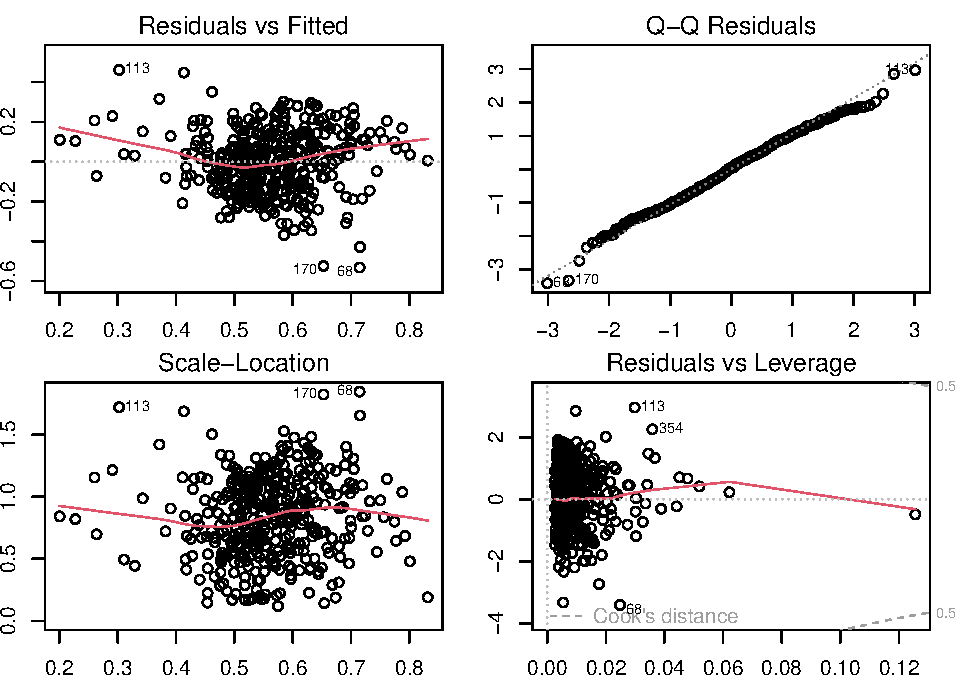
\includegraphics[width=\textwidth]{final-project_files/figure-latex/base-model-plot-1} \caption{ }\label{fig:base-model-plot}
\end{figure}

The residuals look relatively normal from the QQ-plot but there seems to be some clustering in the residuals vs fitted plot and we can see a slight curving.

We then create a basic multiple least squares linear model between the response and our three socioeconomic proxy variables: \emph{Temporary Housing Rate}, \emph{Economic Need Index}, and \emph{Chronic Absenteeism}. We include \emph{Enrollment} as well. The summary statistics of the socieoeconomic model are shown below.

\begin{verbatim}
## 
## Call:
## lm(formula = proxy_formula, data = train)
## 
## Residuals:
##      Min       1Q   Median       3Q      Max 
## -0.45147 -0.08833  0.00416  0.08316  0.31536 
## 
## Coefficients:
##                             Estimate Std. Error t value Pr(>|t|)    
## (Intercept)                1.045e+00  3.776e-02  27.675  < 2e-16 ***
## temp_housing_pct          -5.449e-01  1.193e-01  -4.565 6.72e-06 ***
## economic_need             -4.528e-01  6.124e-02  -7.394 8.97e-13 ***
## val_chronic_absent_hs_all -2.008e-01  3.805e-02  -5.279 2.18e-07 ***
## enrollment                 6.561e-06  9.261e-06   0.708    0.479    
## ---
## Signif. codes:  0 '***' 0.001 '**' 0.01 '*' 0.05 '.' 0.1 ' ' 1
## 
## Residual standard error: 0.1261 on 385 degrees of freedom
## Multiple R-squared:  0.5198, Adjusted R-squared:  0.5149 
## F-statistic: 104.2 on 4 and 385 DF,  p-value: < 2.2e-16
\end{verbatim}

\emph{Enrollment} is not statistically significant, so we remove it and reprint a summary.

\begin{verbatim}
## 
## Call:
## lm(formula = college_rate ~ temp_housing_pct + economic_need + 
##     val_chronic_absent_hs_all, data = train)
## 
## Residuals:
##      Min       1Q   Median       3Q      Max 
## -0.45236 -0.08473  0.00471  0.08199  0.31786 
## 
## Coefficients:
##                           Estimate Std. Error t value Pr(>|t|)    
## (Intercept)                1.05498    0.03494  30.192  < 2e-16 ***
## temp_housing_pct          -0.55304    0.11872  -4.659 4.39e-06 ***
## economic_need             -0.45928    0.06053  -7.588 2.46e-13 ***
## val_chronic_absent_hs_all -0.20141    0.03802  -5.298 1.97e-07 ***
## ---
## Signif. codes:  0 '***' 0.001 '**' 0.01 '*' 0.05 '.' 0.1 ' ' 1
## 
## Residual standard error: 0.1261 on 386 degrees of freedom
## Multiple R-squared:  0.5192, Adjusted R-squared:  0.5155 
## F-statistic:   139 on 3 and 386 DF,  p-value: < 2.2e-16
\end{verbatim}

We find our proxy socioeconomic model produces an adjusted R-squared of \(R^2_{adj} = 0.52\). We also check for multicollinearity within this model. Unlike with the base model based on the survey ratings, we do not expect any such issues with this model.

\begin{table}[H]

\begin{center}
\begin{threeparttable}

\caption{\label{tab:proxy-model-vif-check}Variance Inflation Factors}

\begin{tabular}{ll}
\toprule
 & \multicolumn{1}{c}{VIF Value}\\
\midrule
temp\_housing\_pct & 2.08\\
economic\_need & 2.35\\
val\_chronic\_absent\_hs\_all & 1.26\\
\bottomrule
\end{tabular}

\end{threeparttable}
\end{center}

\end{table}

None of the variance inflation factors are greater than five, so there are no multicollinearity issues to address for this model.

We produce diagnostic plots for the model below.

\begin{figure}[H]
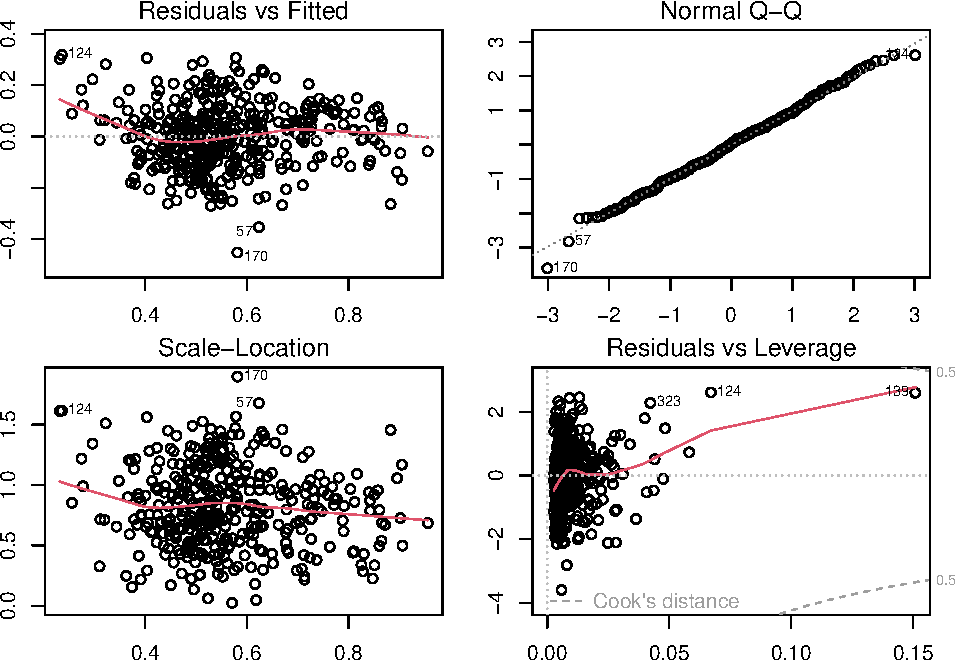
\includegraphics[width=\textwidth]{final-project_files/figure-latex/plot-proxy-model-1} \caption{ }\label{fig:plot-proxy-model}
\end{figure}

We see no strong trend in the residuals vs.~fitted plot, indicating heteroscedasticity. The residuals also look to be normally distributed.

We can also test the assumption of normally-distributed residuals via a \href{https://en.wikipedia.org/wiki/Shapiro–Wilk_test}{Shapiro-Wilk test for normality}. Here we operate with the null \(H_0\) and alternative hypotheses \(H_a\):

\begin{itemize}
\tightlist
\item
  \(H_0\): the error terms of the socioeconomic proxy model come from a normally-distributed population
\item
  \(H_a\): the error terms of the socioeconomic proxy model come from a population that is \textbf{not} normally distributed
\end{itemize}

\begin{verbatim}
## 
##  Shapiro-Wilk normality test
## 
## data:  proxy_model$residuals
## W = 0.99654, p-value = 0.5668
\end{verbatim}

Running a Shapiro test for normality at a 95\% threshold, we receive a p-value of 0.5848, higher than our threshold, so we cannot reject our null hypothesis.

Plotting our proxy model's residuals, we can confirm normality as well visually:
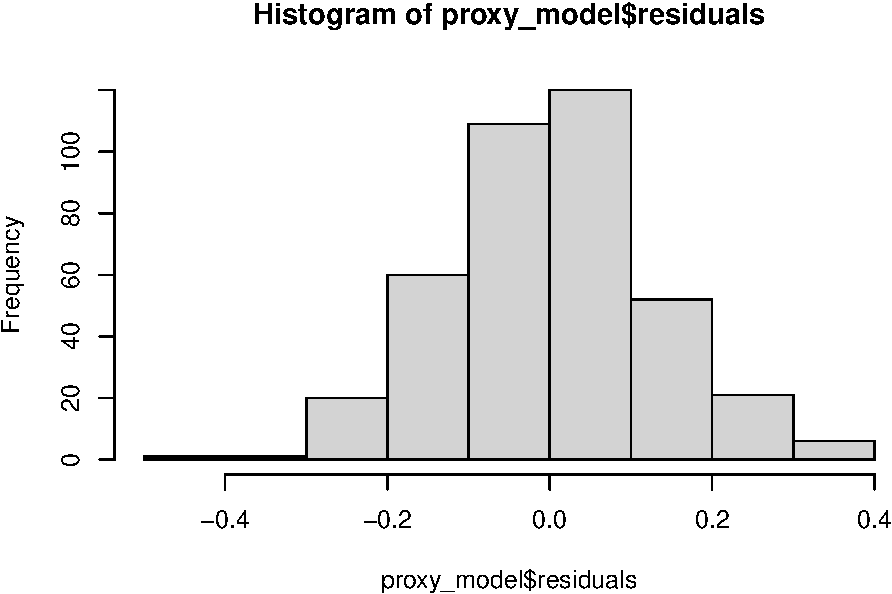
\includegraphics{final-project_files/figure-latex/proxy-residual-plot-1.pdf}

We also fit a weighted-least squares (WLS) model to our proxy variables to account for unqual variances among measurements' residuals. The approach can be used to mitigate the effects of heteroscedastic data when modeling.

\begin{verbatim}
## 
## Call:
## lm(formula = proxy_formula, data = train, weights = weights)
## 
## Weighted Residuals:
##     Min      1Q  Median      3Q     Max 
## -4.4992 -0.8375  0.0549  0.8169  3.1001 
## 
## Coefficients:
##                           Estimate Std. Error t value Pr(>|t|)    
## (Intercept)                1.03959    0.03078  33.776  < 2e-16 ***
## temp_housing_pct          -0.68658    0.12684  -5.413 1.09e-07 ***
## economic_need             -0.41046    0.05692  -7.211 2.96e-12 ***
## val_chronic_absent_hs_all -0.21632    0.03831  -5.646 3.19e-08 ***
## ---
## Signif. codes:  0 '***' 0.001 '**' 0.01 '*' 0.05 '.' 0.1 ' ' 1
## 
## Residual standard error: 1.244 on 386 degrees of freedom
## Multiple R-squared:  0.5589, Adjusted R-squared:  0.5554 
## F-statistic:   163 on 3 and 386 DF,  p-value: < 2.2e-16
\end{verbatim}

\begin{figure}[H]
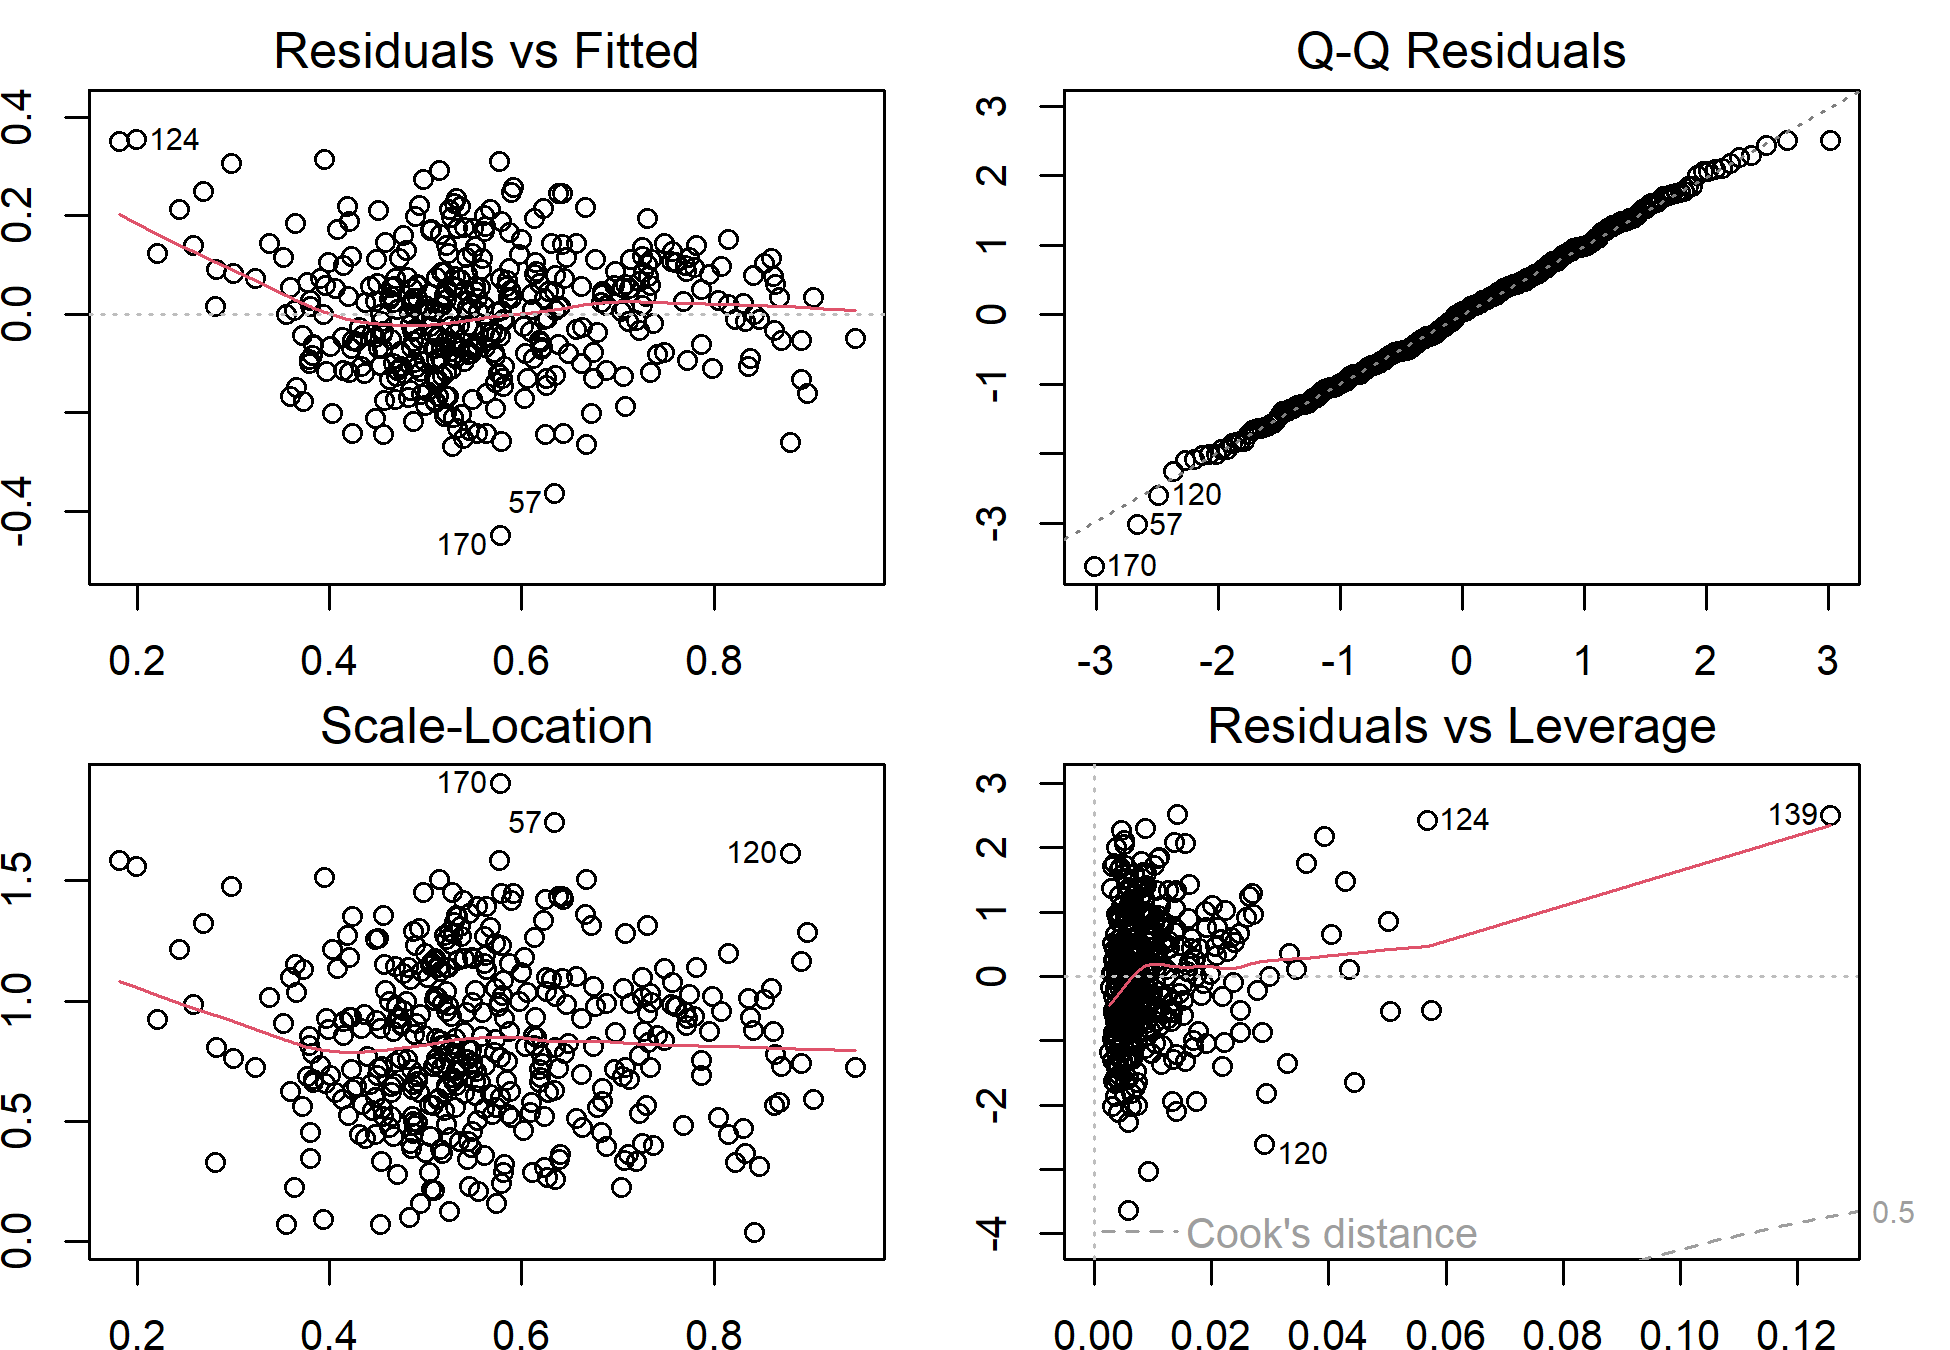
\includegraphics[width=\textwidth]{final-project_files/figure-latex/plot-wls-model-1} \caption{ }\label{fig:plot-wls-model}
\end{figure}

From our diagnostic plots of the WLS model above, we see no general pattern in the \emph{Residuals vs Fitted} plot. In addition, our QQ plot shows general normality behavior, with some behavior off the trendline near the tails of the distribution. Similar to above, we can run a Shapiro test on the residuals of the WLS model to assess normality of residuals, with the same alternative and null hypotheses as above:

\begin{verbatim}
## 
##  Shapiro-Wilk normality test
## 
## data:  wls_model$residuals
## W = 0.99724, p-value = 0.7594
\end{verbatim}

Again, our p-value of 0.7594 indicates that the underlying distribution of residuals is normally distributed,

In the interest of determining whether there are other important variables in the original data that we have not considered, or whether a nonlinear approach could reveal relationships in the data that our linear models have not captured, we train a Support Vector Machine (SVM): Radial Basis (RB) model on centered and scaled data. (Predictors with \texttt{NA} values have been excluded from consideration due to the undesirably large amount of imputation required.)

A summary of the ideal tuning parameters and R-Squared value for the SVM:RB model is below:

\begin{table}[H]

\begin{center}
\begin{threeparttable}

\caption{\label{tab:unnamed-chunk-8}}

\begin{tabular}{llll}
\toprule
Model & \multicolumn{1}{c}{sigma} & \multicolumn{1}{c}{C} & \multicolumn{1}{c}{R-Squared}\\
\midrule
SVM:RB & 0.0244 & 1 & 0.6619\\
\bottomrule
\end{tabular}

\end{threeparttable}
\end{center}

\end{table}

A summary of the estimated feature importance for the ten most important features in this SVM:RB model is below:

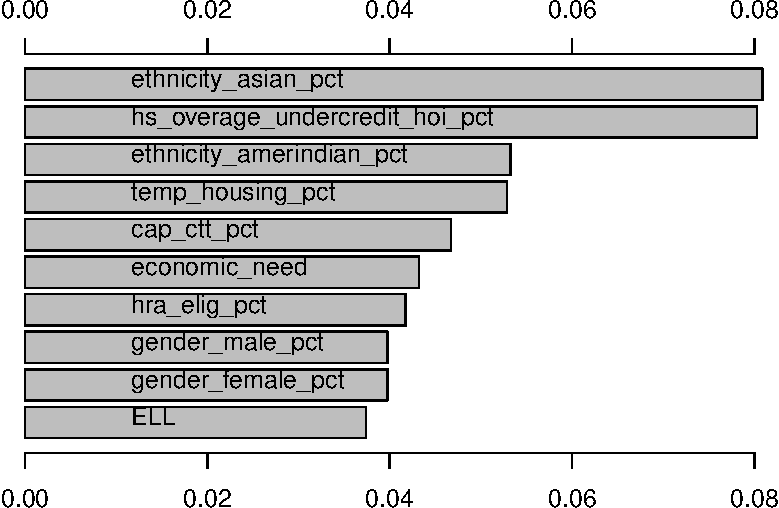
\includegraphics{final-project_files/figure-latex/unnamed-chunk-9-1.pdf}
We can see that the SVM:RB model includes two of our proxy variables in its top ten most important features list: \texttt{temp\_housing\_pct} and \texttt{economic\_need}. However, the single most important feature to the SVM:RB model is \texttt{ethnicity\_asian\_pct}, and the model considers other race and gender percentages important in predicting \texttt{college\_rate} as well. It is not surprising that race and gender play a role in the college persistence rate, and that could be another avenue of analysis. We will not evaluate the SVM:RB further, as our analysis is more focused on linear regression using our selected proxy variables.

Alternatively, we will train a lasso model as a means of feature selection. The ridge-regression penalty \(\lambda\) is fixed at 0, and we will tune over a number of lasso penalties. (Predictors with \texttt{NA} values have again been excluded from consideration due to the undesirably large amount of imputation required.)

A summary of the ideal tuning parameters and R-Squared value for the lasso model is below:

\begin{table}[H]

\begin{center}
\begin{threeparttable}

\caption{\label{tab:unnamed-chunk-10}}

\begin{tabular}{llll}
\toprule
Model & \multicolumn{1}{c}{lambda} & \multicolumn{1}{c}{lasso penalty} & \multicolumn{1}{c}{R-Squared}\\
\midrule
Lasso & 0 & 0.05 & 0.6897\\
\bottomrule
\end{tabular}

\end{threeparttable}
\end{center}

\end{table}

A summary of the estimated feature importance for the twenty-five most important features in this lasso model is below:

\begin{table}[H]

\begin{center}
\begin{threeparttable}

\caption{\label{tab:unnamed-chunk-11}}

\begin{tabular}{ll}
\toprule
Predictor & \multicolumn{1}{c}{Importance}\\
\midrule
hs\_overage\_undercredit\_hoi\_pct & 100.00\\
temp\_housing\_pct & 87.81\\
eni\_hs\_pct\_912 & 76.78\\
economic\_need & 76.78\\
ELL & 69.99\\
hra\_elig\_pct & 68.80\\
val\_attendance\_remote\_hs\_all & 50.39\\
ethnicity\_asian\_pct & 45.16\\
ethnicity\_white\_pct & 40.30\\
IEP & 39.84\\
cap\_ctt\_pct & 33.81\\
n\_credit\_10\_pct\_yr1 & 32.32\\
ethnicity\_hispanic\_pct & 27.05\\
enrollment & 21.46\\
gender\_male\_pct & 21.37\\
gender\_female\_pct & 21.34\\
ethnicity\_black\_pct & 20.52\\
n\_chronic\_absent\_hs\_all & 20.21\\
near\_pct\_white & 20.01\\
n\_attendance\_remote\_hs\_all & 19.79\\
near\_pct\_asian & 19.40\\
n\_attendance\_hs\_all & 17.88\\
near\_pct\_hispanic & 11.95\\
near\_pct\_black & 10.02\\
n\_chronic\_absent\_hs\_alleh & 9.39\\
\bottomrule
\end{tabular}

\end{threeparttable}
\end{center}

\end{table}

In the lasso model, \texttt{temp\_housing\_pct} and \texttt{economic\_need} are more important than any race or gender percentage variables, unlike in the SVM:RB model.

\hypertarget{experimentation-and-results}{%
\section{Experimentation and Results}\label{experimentation-and-results}}

\hypertarget{model-evaluation}{%
\subsubsection{Model Evaluation}\label{model-evaluation}}

We compute the Root mean-squared error (RMSE) for each model on our testing data.

\begin{table}[H]

\begin{center}
\begin{threeparttable}

\caption{\label{tab:RMSE}}

\begin{tabular}{ll}
\toprule
Model & \multicolumn{1}{c}{RMSE}\\
\midrule
Survey Ratings & 0.164516688701194\\
Proxy Variables & 0.142584652490112\\
Weighted Least-Squares & 0.143462660716711\\
\bottomrule
\end{tabular}

\end{threeparttable}
\end{center}

\end{table}

The Proxy Variables model has the lowest RMSE. We can also use the Akaike and Bayesian Information Criterion for evaluating the complexity of our models.

\begin{verbatim}
## 
## Model selection based on AICc:
## 
##                        K    AICc Delta_AICc AICcWt Cum.Wt     LL
## Weighted Least-Squares 5 -508.84       0.00   0.96   0.96 259.50
## Proxy Variables        5 -502.43       6.41   0.04   1.00 256.29
## Survey Ratings         5 -326.91     181.93   0.00   1.00 168.53
\end{verbatim}

\begin{verbatim}
## 
## Model selection based on BIC:
## 
##                        K     BIC Delta_BIC BICWt Cum.Wt     LL
## Weighted Least-Squares 5 -489.16      0.00  0.96   0.96 259.50
## Proxy Variables        5 -482.76      6.41  0.04   1.00 256.29
## Survey Ratings         5 -307.24    181.93  0.00   1.00 168.53
\end{verbatim}

From our tables above, we can see smaller values of corrected AIC (which accounts for smaller sample sizes) from the proxy and WLS models than our base survey rating model. This implies better predictive performance for our WLS and proxy-variable models

\hypertarget{conclusion}{%
\section{Conclusion}\label{conclusion}}

Overall, our model to predict a high school's college persistence rate based on socioeconomic proxy variables outperformed the NYC Schools Open Survey Quality ratings of schools. This is not to say that school ratings based on teacher, student, and parent responses are not valuable inputs. However, they should not be the sole basis upon which educational policy decisions are made, considering the collective socioeconomic factors that most influence a school's performance.

Some limitations of our approach would come from conflation between socioeconomic factors, as well as lacking a more robust imputation method. While our proxy variable model predicts college persistence better than one based off survey ratings, there could be error via omission of unseen variables that are collinear with these inputs. This stems from the availability of data in our source data. We used a \href{https://stefvanbuuren.name/fimd/sec-pmm.html}{\emph{predictive mean matching} imputation method}, native to the \texttt{mice} R package (\emph{Buuren (2018)}). While this allows for realistic imputed values (no imputed value will fall outside the range of observed data), the underlying population distribution of those values could be non-normal.

Future work could include joining in other academic performance metrics (average SAT/ACT scores, etc.) to see if our proxy variables also have predictive power. The dataset provided is indexed on a high school's \emph{district borough number} (DBN), which is present in several \href{https://opendata.cityofnewyork.us}{NYC Open Data} datasets on education in New York City. As mentioned above, joining in other data sources to augment this data could be a good way to address the omission of any variables that better correlate with college persistence rates.

Overall, identifying the factors that most strongly correlate with academic performance and college persistence can improve in educational policy design. In addition, the public availability of educational data through open data platforms only serves to augment the relationships that help this decision-making.

\newpage

\hypertarget{references}{%
\section{References}\label{references}}

\hypertarget{refs}{}
\begin{CSLReferences}{1}{0}
\leavevmode\vadjust pre{\hypertarget{ref-Grades-and-Careers}{}}%
Afarian, R., \& Kleiner, B. (2003). The relationship between grades and career success. \emph{Management Research News}, \emph{26}, 42--51. \url{https://doi.org/10.1108/01409170310783781}

\leavevmode\vadjust pre{\hypertarget{ref-BERNACKI2020103999}{}}%
Bernacki, M. L., Chavez, M. M., \& Uesbeck, P. M. (2020). Predicting achievement and providing support before STEM majors begin to fail. \emph{Computers \& Education}, \emph{158}, 103999. https://doi.org/\url{https://doi.org/10.1016/j.compedu.2020.103999}

\leavevmode\vadjust pre{\hypertarget{ref-Flexible-imputation}{}}%
Buuren, S. van. (2018). \emph{Fleixble imputation of missing data}. Retrieved from \url{https://stefvanbuuren.name/fimd/sec-pmm.html}

\leavevmode\vadjust pre{\hypertarget{ref-NCES-Dropout-Rates}{}}%
Education Statistics, N. C. for. (2008). \emph{Percentage of high school dropouts among persons 16 through 24 years old}. Retrieved from \url{https://nces.ed.gov/programs/digest/d08/tables/dt08_110.asp}

\leavevmode\vadjust pre{\hypertarget{ref-MUSSO202000104}{}}%
Musso, M. F., Cascallar, E. C., Bostani, N., \& Crawford, M. (2020). Identifying reliable predictors of educational outcomes through machine-learning predictive modeling. \emph{Frontiers in Education}, \emph{5}. \url{https://doi.org/10.3389/feduc.2020.00104}

\leavevmode\vadjust pre{\hypertarget{ref-redesign-school-survey}{}}%
New York City Schools, T. R. A. for. (2018). \emph{{R}edesigning the {A}nnual {N}{Y}{C} {S}chool {S}urvey: {L}essons from a {R}esearch-{P}ractice {P}artnership}. \url{https://steinhardt.nyu.edu/sites/default/files/2021-01/Lessons_from_a_Research-Practice_Partnership.pdf}.

\leavevmode\vadjust pre{\hypertarget{ref-roth_meta-analyzing_1996}{}}%
Roth, P. L., BeVier, C. A., Switzer III, F. S., \& Schippmann, J. S. (1996). Meta-analyzing the relationship between grades and job performance. \emph{Journal of Applied Psychology}, \emph{81}(5), 548--556. \url{https://doi.org/10.1037/0021-9010.81.5.548}

\leavevmode\vadjust pre{\hypertarget{ref-CensusBureau_CollegeRates_2023}{}}%
US Census Bureau. (2023). \emph{Census {Cureaur} {Releases} {New} {Educational} {Attainment} {Data}}. Retrieved from \url{https://www.census.gov/newsroom/press-releases/2023/educational-attainment-data.html}

\leavevmode\vadjust pre{\hypertarget{ref-yagci-educational-2022}{}}%
Yağcı, M. (2022). Educational data mining: Prediction of students' academic performance using machine learning algorithms. \emph{Smart Learning Environments}, \emph{9}(1), 11. \url{https://doi.org/10.1186/s40561-022-00192-z}

\end{CSLReferences}

\hypertarget{appendices}{%
\section{Appendices}\label{appendices}}

Below is the code used to generate this report. It's also available on \href{https://github.com/andrewbowen19/businessAnalyticsDataMiningDATA621/main}{GitHub here}.

\begin{Shaded}
\begin{Highlighting}[]
\NormalTok{knitr}\SpecialCharTok{::}\NormalTok{opts\_chunk}\SpecialCharTok{$}\FunctionTok{set}\NormalTok{(}\AttributeTok{echo =} \ConstantTok{FALSE}\NormalTok{, }\AttributeTok{warning =} \ConstantTok{FALSE}\NormalTok{, }\AttributeTok{message =} \ConstantTok{FALSE}\NormalTok{)}
\FunctionTok{library}\NormalTok{(tidyverse)}
\FunctionTok{library}\NormalTok{(gridExtra)}
\FunctionTok{library}\NormalTok{(glue)}
\FunctionTok{library}\NormalTok{(mice)}
\FunctionTok{library}\NormalTok{(corrplot)}
\FunctionTok{library}\NormalTok{(caret)}
\FunctionTok{library}\NormalTok{(modelr)}
\FunctionTok{library}\NormalTok{(}\StringTok{"papaja"}\NormalTok{)}
\FunctionTok{library}\NormalTok{(DataExplorer)}
\FunctionTok{library}\NormalTok{(cowplot)}
\FunctionTok{library}\NormalTok{(car)}
\FunctionTok{library}\NormalTok{(AICcmodavg)}
\FunctionTok{library}\NormalTok{(rminer)}
\FunctionTok{library}\NormalTok{(elasticnet)}
\FunctionTok{r\_refs}\NormalTok{(}\StringTok{"r{-}references.bib"}\NormalTok{)}
\CommentTok{\# Read in our dataset from GitHub}
\CommentTok{\# https://www.opendatanetwork.com/dataset/data.cityofnewyork.us/bm9v{-}cvch}
\NormalTok{df }\OtherTok{\textless{}{-}} \FunctionTok{read.csv}\NormalTok{(}\StringTok{"https://data.cityofnewyork.us/api/views/26je{-}vkp6/rows.csv?date=20231108"}\NormalTok{)}
\NormalTok{label\_cols }\OtherTok{\textless{}{-}} \FunctionTok{c}\NormalTok{(}\StringTok{"dbn"}\NormalTok{, }\StringTok{"school\_name"}\NormalTok{, }\StringTok{"school\_type"}\NormalTok{)}
\CommentTok{\# Convert needed columns to numeric typing}
\NormalTok{df }\OtherTok{\textless{}{-}} \FunctionTok{cbind}\NormalTok{(df[, label\_cols], }\FunctionTok{as.data.frame}\NormalTok{(}\FunctionTok{lapply}\NormalTok{(df[,}\SpecialCharTok{!}\FunctionTok{names}\NormalTok{(df) }\SpecialCharTok{\%in\%}\NormalTok{ label\_cols], as.numeric)))}

\NormalTok{df}\SpecialCharTok{$}\NormalTok{college\_rate }\OtherTok{\textless{}{-}}\NormalTok{ df}\SpecialCharTok{$}\NormalTok{val\_persist3\_4yr\_all}
\NormalTok{df}\SpecialCharTok{$}\NormalTok{economic\_need }\OtherTok{\textless{}{-}}\NormalTok{ df}\SpecialCharTok{$}\NormalTok{eni\_hs\_pct\_912}
\NormalTok{remove }\OtherTok{\textless{}{-}} \FunctionTok{c}\NormalTok{(}\StringTok{"discrete\_columns"}\NormalTok{, }\StringTok{"continuous\_columns"}\NormalTok{,}
            \StringTok{"total\_observations"}\NormalTok{, }\StringTok{"memory\_usage"}\NormalTok{)}
\NormalTok{completeness }\OtherTok{\textless{}{-}} \FunctionTok{introduce}\NormalTok{(df) }\SpecialCharTok{|\textgreater{}}
    \FunctionTok{select}\NormalTok{(}\SpecialCharTok{{-}}\FunctionTok{all\_of}\NormalTok{(remove))}
\FunctionTok{apa\_table}\NormalTok{(}\FunctionTok{t}\NormalTok{(completeness), }\AttributeTok{caption =} \StringTok{"Completeness Summary"}\NormalTok{, }\AttributeTok{placement =} \StringTok{"H"}\NormalTok{)}

\NormalTok{find\_all\_na\_cols }\OtherTok{\textless{}{-}} \ControlFlowTok{function}\NormalTok{(dframe)\{}
\NormalTok{    col\_sums\_na }\OtherTok{\textless{}{-}} \FunctionTok{colSums}\NormalTok{(}\FunctionTok{is.na}\NormalTok{(dframe))}
\NormalTok{    all\_na\_cols }\OtherTok{\textless{}{-}} \FunctionTok{names}\NormalTok{(col\_sums\_na[col\_sums\_na }\SpecialCharTok{==} \FunctionTok{nrow}\NormalTok{(dframe)])}
\NormalTok{    all\_na\_cols}
\NormalTok{\}}
\NormalTok{all\_na\_cols }\OtherTok{\textless{}{-}} \FunctionTok{find\_all\_na\_cols}\NormalTok{(df)}
\NormalTok{df }\OtherTok{\textless{}{-}}\NormalTok{ df }\SpecialCharTok{|\textgreater{}}
    \FunctionTok{select}\NormalTok{(}\SpecialCharTok{{-}}\FunctionTok{all\_of}\NormalTok{(all\_na\_cols))}
\NormalTok{all\_na\_cols }\OtherTok{\textless{}{-}} \FunctionTok{as.data.frame}\NormalTok{(all\_na\_cols)}
\FunctionTok{colnames}\NormalTok{(all\_na\_cols) }\OtherTok{\textless{}{-}} \FunctionTok{c}\NormalTok{(}\StringTok{"All NA Columns"}\NormalTok{)}
\FunctionTok{apa\_table}\NormalTok{(all\_na\_cols, }\AttributeTok{placement =} \StringTok{"H"}\NormalTok{)}

\FunctionTok{set.seed}\NormalTok{(}\DecValTok{42}\NormalTok{)}

\CommentTok{\# Adding a 20\% holdout of our input data for model evaluation later}
\NormalTok{train }\OtherTok{\textless{}{-}} \FunctionTok{subset}\NormalTok{(df[}\FunctionTok{sample}\NormalTok{(}\DecValTok{1}\SpecialCharTok{:}\FunctionTok{nrow}\NormalTok{(df)), ]) }\SpecialCharTok{\%\textgreater{}\%} \FunctionTok{sample\_frac}\NormalTok{(}\FloatTok{0.8}\NormalTok{)}
\NormalTok{train\_svm }\OtherTok{\textless{}{-}}\NormalTok{ train }\SpecialCharTok{|\textgreater{}} \FunctionTok{select}\NormalTok{(}\SpecialCharTok{{-}}\FunctionTok{all\_of}\NormalTok{(}\FunctionTok{c}\NormalTok{(}\StringTok{"dbn"}\NormalTok{, }\StringTok{"school\_name"}\NormalTok{, }\StringTok{"school\_type"}\NormalTok{)))}
\NormalTok{test  }\OtherTok{\textless{}{-}}\NormalTok{ dplyr}\SpecialCharTok{::}\FunctionTok{anti\_join}\NormalTok{(df, train, }\AttributeTok{by =} \StringTok{\textquotesingle{}dbn\textquotesingle{}}\NormalTok{)}
\NormalTok{test\_svm }\OtherTok{\textless{}{-}}\NormalTok{ test }\SpecialCharTok{|\textgreater{}} \FunctionTok{select}\NormalTok{(}\SpecialCharTok{{-}}\FunctionTok{all\_of}\NormalTok{(}\FunctionTok{c}\NormalTok{(}\StringTok{"dbn"}\NormalTok{, }\StringTok{"school\_name"}\NormalTok{, }\StringTok{"school\_type"}\NormalTok{)))}

\NormalTok{cols }\OtherTok{\textless{}{-}} \FunctionTok{c}\NormalTok{(}\StringTok{"survey\_pp\_CT"}\NormalTok{, }\StringTok{"survey\_pp\_RI"}\NormalTok{,}
          \StringTok{"survey\_pp\_ES"}\NormalTok{, }\StringTok{"survey\_pp\_SE"}\NormalTok{,}
          \StringTok{"survey\_pp\_SF"}\NormalTok{, }\StringTok{"survey\_pp\_TR"}\NormalTok{,}
          \StringTok{"temp\_housing\_pct"}\NormalTok{, }\StringTok{"economic\_need"}\NormalTok{,}
          \StringTok{"college\_rate"}\NormalTok{, }\StringTok{"enrollment"}\NormalTok{,}
          \StringTok{"val\_chronic\_absent\_hs\_all"}\NormalTok{)}
\NormalTok{train\_data }\OtherTok{\textless{}{-}}\NormalTok{ train[, cols]}
\NormalTok{p1 }\OtherTok{\textless{}{-}} \FunctionTok{plot\_missing}\NormalTok{(train\_data, }\AttributeTok{missing\_only =} \ConstantTok{FALSE}\NormalTok{,}
                   \AttributeTok{ggtheme =} \FunctionTok{theme\_classic}\NormalTok{(), }\AttributeTok{title =} \StringTok{"Missing Values"}\NormalTok{)}

\CommentTok{\# Plot missing value percentages by cols of interest}
\NormalTok{p1 }\OtherTok{\textless{}{-}}\NormalTok{ p1 }\SpecialCharTok{+} 
    \FunctionTok{scale\_fill\_brewer}\NormalTok{(}\AttributeTok{palette =} \StringTok{"Paired"}\NormalTok{)}
\NormalTok{p1}
\NormalTok{imp }\OtherTok{\textless{}{-}} \FunctionTok{mice}\NormalTok{(train\_data, }\AttributeTok{method=}\StringTok{"pmm"}\NormalTok{, }\AttributeTok{seed=}\DecValTok{42}\NormalTok{, }\AttributeTok{printFlag =} \ConstantTok{FALSE}\NormalTok{)}
\NormalTok{train }\OtherTok{\textless{}{-}} \FunctionTok{complete}\NormalTok{(imp)}
\NormalTok{test\_data }\OtherTok{\textless{}{-}}\NormalTok{ test[, cols]}
\NormalTok{imp }\OtherTok{\textless{}{-}} \FunctionTok{mice}\NormalTok{(test\_data, }\AttributeTok{method=}\StringTok{"pmm"}\NormalTok{, }\AttributeTok{seed=}\DecValTok{42}\NormalTok{, }\AttributeTok{printFlag =} \ConstantTok{FALSE}\NormalTok{)}
\NormalTok{test }\OtherTok{\textless{}{-}} \FunctionTok{complete}\NormalTok{(imp)}
\CommentTok{\# Plot target variable distribution}
\FunctionTok{ggplot}\NormalTok{(train, }\FunctionTok{aes}\NormalTok{(}\AttributeTok{x=}\NormalTok{college\_rate)) }\SpecialCharTok{+} 
    \FunctionTok{geom\_density}\NormalTok{() }\SpecialCharTok{+} 
    \FunctionTok{labs}\NormalTok{(}\AttributeTok{x=}\StringTok{"4{-}Year College Persistence Rate"}\NormalTok{,}
         \AttributeTok{y=}\StringTok{"Density of NYC High Schools"}\NormalTok{,}
         \AttributeTok{title=}\StringTok{"Average 4{-}Year College Persistence Rates: NYC High Schools 2020{-}2021"}\NormalTok{,}
         \AttributeTok{caption=}\StringTok{"The average NYC high school sees \textasciitilde{}50\% of students go on to have 4{-}year college persistence."}\NormalTok{)}

\FunctionTok{theme\_set}\NormalTok{(}\FunctionTok{theme\_apa}\NormalTok{())}
\CommentTok{\# Renaming training dataframe for correlation plot}
\NormalTok{train\_renamed }\OtherTok{\textless{}{-}}\NormalTok{ train }\SpecialCharTok{\%\textgreater{}\%}
  \FunctionTok{rename}\NormalTok{(}\StringTok{"Collaborative Teaching"}\OtherTok{=}\NormalTok{survey\_pp\_CT,}
         \StringTok{"Rigorous Instruction"}\OtherTok{=}\NormalTok{survey\_pp\_RI,}
         \StringTok{"Supportive Env"}\OtherTok{=}\NormalTok{survey\_pp\_SE,}
         \StringTok{"Effective Leadership"}\OtherTok{=}\NormalTok{survey\_pp\_ES,}
         \StringTok{"Family{-}Community Ties"}\OtherTok{=}\NormalTok{survey\_pp\_SF,}
         \StringTok{"Trust"}\OtherTok{=}\NormalTok{survey\_pp\_TR,}
         \StringTok{"Temporary Housing Pct"}\OtherTok{=}\NormalTok{temp\_housing\_pct,}
         \StringTok{"Economic Need"}\OtherTok{=}\NormalTok{economic\_need,}
         \StringTok{"College Persistence"}\OtherTok{=}\NormalTok{college\_rate,}
         \StringTok{"Enrollment"}\OtherTok{=}\NormalTok{enrollment,}
         \StringTok{"Chronic Absenteeism"}\OtherTok{=}\NormalTok{val\_chronic\_absent\_hs\_all)}

\CommentTok{\# Create correlation plot between vars of interest}
\NormalTok{corMatrix }\OtherTok{\textless{}{-}} \FunctionTok{cor}\NormalTok{(train\_renamed)}
\FunctionTok{corrplot}\NormalTok{(corMatrix, }\AttributeTok{method=}\StringTok{"color"}\NormalTok{, }\AttributeTok{type=}\StringTok{"lower"}\NormalTok{, }\AttributeTok{tl.col=}\StringTok{"black"}\NormalTok{, }\AttributeTok{addCoef.col =} \StringTok{"black"}\NormalTok{, }\AttributeTok{tl.cex =} \FloatTok{0.7}\NormalTok{, }\AttributeTok{number.cex =} \FloatTok{0.6}\NormalTok{)}

\CommentTok{\# Plot temp housing rates}
\NormalTok{pa }\OtherTok{\textless{}{-}} \FunctionTok{ggplot}\NormalTok{(train, }\FunctionTok{aes}\NormalTok{(}\AttributeTok{x=}\NormalTok{temp\_housing\_pct)) }\SpecialCharTok{+}
    \FunctionTok{geom\_density}\NormalTok{() }\SpecialCharTok{+}
    \FunctionTok{labs}\NormalTok{(}\AttributeTok{x=}\StringTok{"\% Students Temp Housing"}\NormalTok{, }\AttributeTok{y=}\StringTok{"Density"}\NormalTok{)}
\CommentTok{\# Plot economic need index}
\NormalTok{pb }\OtherTok{\textless{}{-}} \FunctionTok{ggplot}\NormalTok{(train, }\FunctionTok{aes}\NormalTok{(}\AttributeTok{x=}\NormalTok{economic\_need)) }\SpecialCharTok{+}
    \FunctionTok{geom\_density}\NormalTok{() }\SpecialCharTok{+}
    \FunctionTok{labs}\NormalTok{(}\AttributeTok{x=}\StringTok{"Economic Need Index"}\NormalTok{, }\AttributeTok{y=}\StringTok{"Density"}\NormalTok{)}
\CommentTok{\# Plot enrollment}
\NormalTok{pc }\OtherTok{\textless{}{-}} \FunctionTok{ggplot}\NormalTok{(train, }\FunctionTok{aes}\NormalTok{(}\AttributeTok{x=}\NormalTok{enrollment)) }\SpecialCharTok{+}
    \FunctionTok{geom\_density}\NormalTok{() }\SpecialCharTok{+}
    \FunctionTok{labs}\NormalTok{(}\AttributeTok{x=}\StringTok{"Enrollment"}\NormalTok{, }\AttributeTok{y=}\StringTok{"Density"}\NormalTok{)}
\CommentTok{\# Plot chronic absenteeism}
\NormalTok{pd }\OtherTok{\textless{}{-}} \FunctionTok{ggplot}\NormalTok{(train, }\FunctionTok{aes}\NormalTok{(}\AttributeTok{x=}\NormalTok{val\_chronic\_absent\_hs\_all)) }\SpecialCharTok{+}
    \FunctionTok{geom\_density}\NormalTok{() }\SpecialCharTok{+}
    \FunctionTok{labs}\NormalTok{(}\AttributeTok{x=}\StringTok{"Chronic Absenteeism"}\NormalTok{, }\AttributeTok{y=}\StringTok{"Density"}\NormalTok{)}
\NormalTok{p }\OtherTok{\textless{}{-}} \FunctionTok{plot\_grid}\NormalTok{(pa, pb, pc, pd, }\AttributeTok{nrow =} \DecValTok{2}\NormalTok{, }\AttributeTok{ncol =} \DecValTok{2}\NormalTok{, }\AttributeTok{align =} \StringTok{"hv"}\NormalTok{, }\AttributeTok{axis =} \StringTok{"t"}\NormalTok{)}
\NormalTok{p}

\CommentTok{\# Plot temp housing percentage vs college persistence rate}
\NormalTok{pa }\OtherTok{\textless{}{-}} \FunctionTok{ggplot}\NormalTok{(train, }\FunctionTok{aes}\NormalTok{(}\AttributeTok{x=}\NormalTok{temp\_housing\_pct, }\AttributeTok{y=}\NormalTok{college\_rate)) }\SpecialCharTok{+}
  \FunctionTok{geom\_point}\NormalTok{() }\SpecialCharTok{+}
  \FunctionTok{labs}\NormalTok{(}\AttributeTok{x=}\StringTok{"\% Students in Temp Housing"}\NormalTok{,}
       \AttributeTok{y=}\StringTok{"College Persist"}\NormalTok{)}
\CommentTok{\# Plot ENI vs college persistence rate}
\NormalTok{pb }\OtherTok{\textless{}{-}} \FunctionTok{ggplot}\NormalTok{(train, }\FunctionTok{aes}\NormalTok{(}\AttributeTok{x=}\NormalTok{economic\_need, }\AttributeTok{y=}\NormalTok{college\_rate)) }\SpecialCharTok{+}
  \FunctionTok{geom\_point}\NormalTok{() }\SpecialCharTok{+}
  \FunctionTok{labs}\NormalTok{(}\AttributeTok{x=}\StringTok{"Economic Need Index"}\NormalTok{,}
       \AttributeTok{y=}\StringTok{"College Persist"}\NormalTok{)}
\NormalTok{pc }\OtherTok{\textless{}{-}} \FunctionTok{ggplot}\NormalTok{(train, }\FunctionTok{aes}\NormalTok{(}\AttributeTok{x=}\NormalTok{enrollment, }\AttributeTok{y=}\NormalTok{college\_rate)) }\SpecialCharTok{+}
  \FunctionTok{geom\_point}\NormalTok{() }\SpecialCharTok{+}
  \FunctionTok{labs}\NormalTok{(}\AttributeTok{x=}\StringTok{"Enrollment"}\NormalTok{,}
       \AttributeTok{y=}\StringTok{"College Persist"}\NormalTok{)}
\NormalTok{pd }\OtherTok{\textless{}{-}} \FunctionTok{ggplot}\NormalTok{(train, }\FunctionTok{aes}\NormalTok{(}\AttributeTok{x=}\NormalTok{val\_chronic\_absent\_hs\_all, }\AttributeTok{y=}\NormalTok{college\_rate)) }\SpecialCharTok{+}
  \FunctionTok{geom\_point}\NormalTok{() }\SpecialCharTok{+}
  \FunctionTok{labs}\NormalTok{(}\AttributeTok{x=}\StringTok{"Chronic Absenteeism"}\NormalTok{,}
       \AttributeTok{y=}\StringTok{"College Persist"}\NormalTok{)}
\NormalTok{p }\OtherTok{\textless{}{-}} \FunctionTok{plot\_grid}\NormalTok{(pa, pb, pc, pd, }\AttributeTok{nrow =} \DecValTok{2}\NormalTok{, }\AttributeTok{ncol =} \DecValTok{2}\NormalTok{, }\AttributeTok{align =} \StringTok{"hv"}\NormalTok{, }\AttributeTok{axis =} \StringTok{"t"}\NormalTok{)}
\NormalTok{p}

\NormalTok{base\_formula }\OtherTok{\textless{}{-}}\NormalTok{ college\_rate }\SpecialCharTok{\textasciitilde{}}\NormalTok{ survey\_pp\_CT }\SpecialCharTok{+}\NormalTok{ survey\_pp\_RI }\SpecialCharTok{+}\NormalTok{ survey\_pp\_SE }\SpecialCharTok{+}\NormalTok{ survey\_pp\_ES }\SpecialCharTok{+}\NormalTok{ survey\_pp\_SF }\SpecialCharTok{+}\NormalTok{ survey\_pp\_TR}
\NormalTok{rating\_model }\OtherTok{\textless{}{-}} \FunctionTok{lm}\NormalTok{(base\_formula,}
\NormalTok{                   train)}
\FunctionTok{summary}\NormalTok{(rating\_model)}

\NormalTok{rating\_model }\OtherTok{\textless{}{-}} \FunctionTok{update}\NormalTok{(rating\_model, }\SpecialCharTok{\textasciitilde{}}\NormalTok{ . }\SpecialCharTok{{-}}\NormalTok{ survey\_pp\_CT }\SpecialCharTok{{-}}\NormalTok{ survey\_pp\_SF }\SpecialCharTok{{-}}\NormalTok{ survey\_pp\_TR)}
\FunctionTok{summary}\NormalTok{(rating\_model)}

\NormalTok{vif\_df }\OtherTok{\textless{}{-}} \FunctionTok{as.data.frame}\NormalTok{(}\FunctionTok{vif}\NormalTok{(rating\_model))}
\FunctionTok{colnames}\NormalTok{(vif\_df) }\OtherTok{\textless{}{-}} \FunctionTok{c}\NormalTok{(}\StringTok{"VIF Value"}\NormalTok{)}
\FunctionTok{apa\_table}\NormalTok{(vif\_df, }\AttributeTok{caption =} \StringTok{"Variance Inflation Factors"}\NormalTok{, }\AttributeTok{placement =} \StringTok{"H"}\NormalTok{)}
\FunctionTok{par}\NormalTok{(}\AttributeTok{mfrow=}\FunctionTok{c}\NormalTok{(}\DecValTok{2}\NormalTok{,}\DecValTok{2}\NormalTok{))}
\FunctionTok{par}\NormalTok{(}\AttributeTok{mai=}\FunctionTok{c}\NormalTok{(.}\DecValTok{3}\NormalTok{,.}\DecValTok{3}\NormalTok{,.}\DecValTok{3}\NormalTok{,.}\DecValTok{3}\NormalTok{))}
\FunctionTok{plot}\NormalTok{(rating\_model)}

\CommentTok{\# Create OLS linear model based on our proxy variables: no transforms}
\NormalTok{proxy\_formula }\OtherTok{\textless{}{-}}\NormalTok{ college\_rate }\SpecialCharTok{\textasciitilde{}}\NormalTok{ temp\_housing\_pct }\SpecialCharTok{+}\NormalTok{ economic\_need }\SpecialCharTok{+}\NormalTok{ val\_chronic\_absent\_hs\_all }\SpecialCharTok{+}\NormalTok{ enrollment}
\NormalTok{proxy\_model }\OtherTok{\textless{}{-}} \FunctionTok{lm}\NormalTok{(proxy\_formula, train)}
\FunctionTok{summary}\NormalTok{(proxy\_model)}

\NormalTok{proxy\_model }\OtherTok{\textless{}{-}} \FunctionTok{update}\NormalTok{(proxy\_model, }\SpecialCharTok{\textasciitilde{}}\NormalTok{ . }\SpecialCharTok{{-}}\NormalTok{ enrollment)}
\FunctionTok{summary}\NormalTok{(proxy\_model)}

\NormalTok{vif\_df }\OtherTok{\textless{}{-}} \FunctionTok{as.data.frame}\NormalTok{(}\FunctionTok{vif}\NormalTok{(proxy\_model))}
\FunctionTok{colnames}\NormalTok{(vif\_df) }\OtherTok{\textless{}{-}} \FunctionTok{c}\NormalTok{(}\StringTok{"VIF Value"}\NormalTok{)}
\FunctionTok{apa\_table}\NormalTok{(vif\_df, }\AttributeTok{caption =} \StringTok{"Variance Inflation Factors"}\NormalTok{, }\AttributeTok{placement =} \StringTok{"H"}\NormalTok{)}

\FunctionTok{par}\NormalTok{(}\AttributeTok{mfrow=}\FunctionTok{c}\NormalTok{(}\DecValTok{2}\NormalTok{,}\DecValTok{2}\NormalTok{))}
\FunctionTok{par}\NormalTok{(}\AttributeTok{mai=}\FunctionTok{c}\NormalTok{(.}\DecValTok{3}\NormalTok{,.}\DecValTok{3}\NormalTok{,.}\DecValTok{3}\NormalTok{,.}\DecValTok{3}\NormalTok{))}
\FunctionTok{plot}\NormalTok{(proxy\_model)}

\CommentTok{\# Test proxy model for normality of residuals}
\FunctionTok{shapiro.test}\NormalTok{(proxy\_model}\SpecialCharTok{$}\NormalTok{residuals)}
\FunctionTok{hist}\NormalTok{(proxy\_model}\SpecialCharTok{$}\NormalTok{residuals, }\AttributeTok{xlab=}\StringTok{"Proxy Model Residuals"}\NormalTok{)}
\CommentTok{\# Calculating weights for WLS}
\NormalTok{weights }\OtherTok{\textless{}{-}} \DecValTok{1} \SpecialCharTok{/} \FunctionTok{lm}\NormalTok{(}\FunctionTok{abs}\NormalTok{(proxy\_model}\SpecialCharTok{$}\NormalTok{residuals) }\SpecialCharTok{\textasciitilde{}}\NormalTok{ proxy\_model}\SpecialCharTok{$}\NormalTok{fitted.values)}\SpecialCharTok{$}\NormalTok{fitted.values}\SpecialCharTok{\^{}}\DecValTok{2}

\CommentTok{\#perform weighted least squares regression}
\NormalTok{proxy\_formula }\OtherTok{\textless{}{-}}\NormalTok{ proxy\_model}\SpecialCharTok{$}\NormalTok{call}\SpecialCharTok{$}\NormalTok{formula}
\NormalTok{wls\_model }\OtherTok{\textless{}{-}} \FunctionTok{lm}\NormalTok{(proxy\_formula, }\AttributeTok{data =}\NormalTok{ train, }\AttributeTok{weights=}\NormalTok{weights)}

\FunctionTok{summary}\NormalTok{(wls\_model)}
\FunctionTok{par}\NormalTok{(}\AttributeTok{mfrow=}\FunctionTok{c}\NormalTok{(}\DecValTok{2}\NormalTok{,}\DecValTok{2}\NormalTok{))}
\FunctionTok{par}\NormalTok{(}\AttributeTok{mai=}\FunctionTok{c}\NormalTok{(.}\DecValTok{3}\NormalTok{,.}\DecValTok{3}\NormalTok{,.}\DecValTok{3}\NormalTok{,.}\DecValTok{3}\NormalTok{))}
\FunctionTok{plot}\NormalTok{(wls\_model)}
\FunctionTok{shapiro.test}\NormalTok{(wls\_model}\SpecialCharTok{$}\NormalTok{residuals)}
\NormalTok{na\_count }\OtherTok{\textless{}{-}}\FunctionTok{sapply}\NormalTok{(train\_svm, }\ControlFlowTok{function}\NormalTok{(y) }\FunctionTok{sum}\NormalTok{(}\FunctionTok{length}\NormalTok{(}\FunctionTok{which}\NormalTok{(}\FunctionTok{is.na}\NormalTok{(y)))))}
\NormalTok{na\_count }\OtherTok{\textless{}{-}} \FunctionTok{data.frame}\NormalTok{(na\_count)}
\NormalTok{na\_count }\OtherTok{\textless{}{-}}\NormalTok{ na\_count }\SpecialCharTok{|\textgreater{}}
    \FunctionTok{filter}\NormalTok{(na\_count }\SpecialCharTok{==} \DecValTok{0}\NormalTok{)}
\NormalTok{incl }\OtherTok{\textless{}{-}} \FunctionTok{rownames}\NormalTok{(na\_count)}
\NormalTok{train\_svm }\OtherTok{\textless{}{-}}\NormalTok{ train\_svm }\SpecialCharTok{|\textgreater{}}
    \FunctionTok{drop\_na}\NormalTok{(college\_rate)}
\NormalTok{svmRBTuned }\OtherTok{\textless{}{-}} \FunctionTok{train}\NormalTok{(train\_svm }\SpecialCharTok{|\textgreater{}} \FunctionTok{select}\NormalTok{(}\FunctionTok{all\_of}\NormalTok{(incl)), train\_svm}\SpecialCharTok{$}\NormalTok{college\_rate,}
                    \AttributeTok{method =} \StringTok{"svmRadial"}\NormalTok{,}
                    \AttributeTok{preProc =} \FunctionTok{c}\NormalTok{(}\StringTok{"center"}\NormalTok{, }\StringTok{"scale"}\NormalTok{),}
                    \AttributeTok{tuneLength =} \DecValTok{14}\NormalTok{,}
                    \AttributeTok{trControl =} \FunctionTok{trainControl}\NormalTok{(}\AttributeTok{method =} \StringTok{"cv"}\NormalTok{))}

\NormalTok{svm\_summ }\OtherTok{\textless{}{-}} \FunctionTok{c}\NormalTok{(}\StringTok{"SVM:RB"}\NormalTok{,}
             \FunctionTok{round}\NormalTok{(svmRBTuned}\SpecialCharTok{$}\NormalTok{bestTune}\SpecialCharTok{$}\NormalTok{sigma, }\DecValTok{4}\NormalTok{),}
\NormalTok{             svmRBTuned}\SpecialCharTok{$}\NormalTok{bestTune}\SpecialCharTok{$}\NormalTok{C,}
             \FunctionTok{round}\NormalTok{(svmRBTuned}\SpecialCharTok{$}\NormalTok{results }\SpecialCharTok{|\textgreater{}}
                 \FunctionTok{filter}\NormalTok{(C }\SpecialCharTok{==}\NormalTok{ svmRBTuned}\SpecialCharTok{$}\NormalTok{bestTune}\SpecialCharTok{$}\NormalTok{C) }\SpecialCharTok{|\textgreater{}}
                 \FunctionTok{select}\NormalTok{(Rsquared) }\SpecialCharTok{|\textgreater{}} \FunctionTok{as.numeric}\NormalTok{(), }\DecValTok{4}\NormalTok{))}
\NormalTok{svm\_summ }\OtherTok{\textless{}{-}} \FunctionTok{as.data.frame}\NormalTok{(}\FunctionTok{t}\NormalTok{(svm\_summ))}
\NormalTok{cols }\OtherTok{\textless{}{-}} \FunctionTok{c}\NormalTok{(}\StringTok{"Model"}\NormalTok{, }\StringTok{"sigma"}\NormalTok{, }\StringTok{"C"}\NormalTok{, }\StringTok{"R{-}Squared"}\NormalTok{)}
\FunctionTok{colnames}\NormalTok{(svm\_summ) }\OtherTok{\textless{}{-}}\NormalTok{ cols}
\FunctionTok{apa\_table}\NormalTok{(svm\_summ, }\AttributeTok{placement =} \StringTok{"H"}\NormalTok{)}

\NormalTok{y }\OtherTok{\textless{}{-}}\NormalTok{ train\_svm}\SpecialCharTok{$}\NormalTok{college\_rate}
\FunctionTok{names}\NormalTok{(y) }\OtherTok{\textless{}{-}} \StringTok{"y"}
\NormalTok{dat }\OtherTok{=} \FunctionTok{cbind}\NormalTok{(train\_svm }\SpecialCharTok{|\textgreater{}} \FunctionTok{select}\NormalTok{(}\FunctionTok{all\_of}\NormalTok{(incl)), y)}
\NormalTok{svmRBFit }\OtherTok{\textless{}{-}} \FunctionTok{fit}\NormalTok{(y}\SpecialCharTok{\textasciitilde{}}\NormalTok{., }\AttributeTok{data =}\NormalTok{ dat, }\AttributeTok{model =} \StringTok{"svm"}\NormalTok{,}
               \AttributeTok{kpar =} \FunctionTok{list}\NormalTok{(}\AttributeTok{sigma =} \FloatTok{0.0244}\NormalTok{), }\AttributeTok{C =} \DecValTok{1}\NormalTok{)}
\NormalTok{svmRB.imp }\OtherTok{\textless{}{-}} \FunctionTok{Importance}\NormalTok{(svmRBFit, }\AttributeTok{data =}\NormalTok{ dat)}
\NormalTok{L }\OtherTok{=} \FunctionTok{list}\NormalTok{(}\AttributeTok{runs =} \DecValTok{1}\NormalTok{,}\AttributeTok{sen =} \FunctionTok{t}\NormalTok{(svmRB.imp}\SpecialCharTok{$}\NormalTok{imp),}
         \AttributeTok{sresponses =}\NormalTok{ svmRB.imp}\SpecialCharTok{$}\NormalTok{sresponses)}
\NormalTok{sen\_vec }\OtherTok{\textless{}{-}} \FunctionTok{as.numeric}\NormalTok{(L[[}\StringTok{"sen"}\NormalTok{]])}
\NormalTok{copy }\OtherTok{\textless{}{-}}\NormalTok{ L}
\NormalTok{delete }\OtherTok{\textless{}{-}} \FunctionTok{c}\NormalTok{()}
\NormalTok{sort }\OtherTok{\textless{}{-}} \FunctionTok{sort}\NormalTok{(sen\_vec, }\AttributeTok{decreasing =} \ConstantTok{TRUE}\NormalTok{)}
\ControlFlowTok{for}\NormalTok{ (i }\ControlFlowTok{in} \DecValTok{1}\SpecialCharTok{:}\FunctionTok{length}\NormalTok{(sen\_vec))\{}
    \ControlFlowTok{if}\NormalTok{ (sen\_vec[i] }\SpecialCharTok{\textgreater{}}\NormalTok{ sort[}\DecValTok{11}\NormalTok{])\{}
        \ControlFlowTok{next}
\NormalTok{    \}}\ControlFlowTok{else}\NormalTok{\{}
\NormalTok{        delete }\OtherTok{\textless{}{-}} \FunctionTok{append}\NormalTok{(delete, i)}
\NormalTok{    \}}
\NormalTok{\}}
\NormalTok{copy[[}\StringTok{"sen"}\NormalTok{]] }\OtherTok{\textless{}{-}} \FunctionTok{t}\NormalTok{(}\FunctionTok{as.matrix}\NormalTok{(copy[[}\StringTok{"sen"}\NormalTok{]][, }\SpecialCharTok{{-}}\NormalTok{delete]))}
\NormalTok{copy[[}\StringTok{"sresponses"}\NormalTok{]] }\OtherTok{\textless{}{-}}\NormalTok{ copy[[}\StringTok{"sresponses"}\NormalTok{]][}\SpecialCharTok{{-}}\NormalTok{delete]}
\NormalTok{names }\OtherTok{\textless{}{-}} \FunctionTok{c}\NormalTok{()}
\ControlFlowTok{for}\NormalTok{ (i }\ControlFlowTok{in} \DecValTok{1}\SpecialCharTok{:}\FunctionTok{length}\NormalTok{(copy[[}\StringTok{"sresponses"}\NormalTok{]]))\{}
\NormalTok{    n }\OtherTok{\textless{}{-}}\NormalTok{ copy[[}\StringTok{"sresponses"}\NormalTok{]][[i]][[}\StringTok{"n"}\NormalTok{]]}
\NormalTok{    names }\OtherTok{\textless{}{-}} \FunctionTok{append}\NormalTok{(names, n)}
\NormalTok{\}}
\FunctionTok{mgraph}\NormalTok{(copy, }\AttributeTok{graph =} \StringTok{"IMP"}\NormalTok{, }\AttributeTok{leg =}\NormalTok{ names, }\AttributeTok{col =} \StringTok{"gray"}\NormalTok{,}
       \AttributeTok{PDF =} \StringTok{""}\NormalTok{)}

\NormalTok{train\_lasso }\OtherTok{\textless{}{-}}\NormalTok{ train\_svm}
\NormalTok{lassoGrid }\OtherTok{\textless{}{-}} \FunctionTok{expand.grid}\NormalTok{(}\AttributeTok{.lambda =} \FunctionTok{c}\NormalTok{(}\DecValTok{0}\NormalTok{),}
                         \AttributeTok{.fraction =} \FunctionTok{seq}\NormalTok{(.}\DecValTok{05}\NormalTok{, }\DecValTok{1}\NormalTok{, }\AttributeTok{length =} \DecValTok{20}\NormalTok{))}
\NormalTok{ctrl }\OtherTok{\textless{}{-}} \FunctionTok{trainControl}\NormalTok{(}\AttributeTok{method =} \StringTok{"cv"}\NormalTok{, }\AttributeTok{number =} \DecValTok{10}\NormalTok{)}
\NormalTok{lassoTune }\OtherTok{\textless{}{-}} \FunctionTok{train}\NormalTok{(train\_lasso }\SpecialCharTok{|\textgreater{}} \FunctionTok{select}\NormalTok{(}\FunctionTok{all\_of}\NormalTok{(incl)),}
\NormalTok{                   train\_lasso}\SpecialCharTok{$}\NormalTok{college\_rate,}
                   \AttributeTok{method =} \StringTok{"enet"}\NormalTok{,}
                   \AttributeTok{tuneGrid =}\NormalTok{ lassoGrid,}
                   \AttributeTok{trControl =}\NormalTok{ ctrl,}
                   \AttributeTok{preProc =} \FunctionTok{c}\NormalTok{(}\StringTok{"center"}\NormalTok{, }\StringTok{"scale"}\NormalTok{))}

\NormalTok{lasso\_summ }\OtherTok{\textless{}{-}} \FunctionTok{c}\NormalTok{(}\StringTok{"Lasso"}\NormalTok{,}
\NormalTok{             lassoTune}\SpecialCharTok{$}\NormalTok{bestTune}\SpecialCharTok{$}\NormalTok{lambda,}
\NormalTok{             lassoTune}\SpecialCharTok{$}\NormalTok{bestTune}\SpecialCharTok{$}\NormalTok{fraction,}
             \FunctionTok{round}\NormalTok{(lassoTune}\SpecialCharTok{$}\NormalTok{results }\SpecialCharTok{|\textgreater{}}
                 \FunctionTok{filter}\NormalTok{(fraction }\SpecialCharTok{==}\NormalTok{ lassoTune}\SpecialCharTok{$}\NormalTok{bestTune}\SpecialCharTok{$}\NormalTok{fraction) }\SpecialCharTok{|\textgreater{}}
                 \FunctionTok{select}\NormalTok{(Rsquared) }\SpecialCharTok{|\textgreater{}} \FunctionTok{as.numeric}\NormalTok{(), }\DecValTok{4}\NormalTok{))}
\NormalTok{lasso\_summ }\OtherTok{\textless{}{-}} \FunctionTok{as.data.frame}\NormalTok{(}\FunctionTok{t}\NormalTok{(lasso\_summ))}
\NormalTok{cols }\OtherTok{\textless{}{-}} \FunctionTok{c}\NormalTok{(}\StringTok{"Model"}\NormalTok{, }\StringTok{"lambda"}\NormalTok{, }\StringTok{"lasso penalty"}\NormalTok{, }\StringTok{"R{-}Squared"}\NormalTok{)}
\FunctionTok{colnames}\NormalTok{(lasso\_summ) }\OtherTok{\textless{}{-}}\NormalTok{ cols}
\FunctionTok{apa\_table}\NormalTok{(lasso\_summ, }\AttributeTok{placement =} \StringTok{"H"}\NormalTok{)}

\NormalTok{lasso\_imp }\OtherTok{\textless{}{-}} \FunctionTok{varImp}\NormalTok{(lassoTune, }\AttributeTok{scale =} \ConstantTok{TRUE}\NormalTok{)}
\NormalTok{cols }\OtherTok{\textless{}{-}} \FunctionTok{c}\NormalTok{(}\StringTok{"Predictor"}\NormalTok{, }\StringTok{"Importance"}\NormalTok{)}
\NormalTok{lasso\_imp }\OtherTok{\textless{}{-}}\NormalTok{ lasso\_imp}\SpecialCharTok{$}\NormalTok{importance }\SpecialCharTok{|\textgreater{}}
    \FunctionTok{rownames\_to\_column}\NormalTok{()}
\FunctionTok{colnames}\NormalTok{(lasso\_imp) }\OtherTok{\textless{}{-}}\NormalTok{ cols}
\NormalTok{lasso\_imp }\OtherTok{\textless{}{-}}\NormalTok{ lasso\_imp }\SpecialCharTok{|\textgreater{}}
    \FunctionTok{arrange}\NormalTok{(}\FunctionTok{desc}\NormalTok{(Importance)) }\SpecialCharTok{|\textgreater{}}
    \FunctionTok{top\_n}\NormalTok{(}\DecValTok{25}\NormalTok{)}
\FunctionTok{apa\_table}\NormalTok{(lasso\_imp, }\AttributeTok{placement =} \StringTok{"H"}\NormalTok{)}

\CommentTok{\# Compute RMSE for each model on our testing data}
\NormalTok{model\_names }\OtherTok{\textless{}{-}} \FunctionTok{c}\NormalTok{(}\StringTok{"Survey Ratings"}\NormalTok{, }\StringTok{"Proxy Variables"}\NormalTok{, }\StringTok{"Weighted Least{-}Squares"}\NormalTok{)}
\NormalTok{rmse\_summ }\OtherTok{\textless{}{-}} \FunctionTok{c}\NormalTok{(}\FunctionTok{rmse}\NormalTok{(rating\_model, test),}
\NormalTok{               modelr}\SpecialCharTok{::}\FunctionTok{rmse}\NormalTok{(proxy\_model, test),}
\NormalTok{               modelr}\SpecialCharTok{::}\FunctionTok{rmse}\NormalTok{(wls\_model, test))}
\NormalTok{rmse\_summ }\OtherTok{\textless{}{-}} \FunctionTok{as.data.frame}\NormalTok{(}\FunctionTok{cbind}\NormalTok{(model\_names, rmse\_summ))}
\NormalTok{cols }\OtherTok{\textless{}{-}} \FunctionTok{c}\NormalTok{(}\StringTok{"Model"}\NormalTok{, }\StringTok{"RMSE"}\NormalTok{)}
\FunctionTok{colnames}\NormalTok{(rmse\_summ) }\OtherTok{\textless{}{-}}\NormalTok{ cols}
\FunctionTok{apa\_table}\NormalTok{(rmse\_summ, }\AttributeTok{placement =} \StringTok{"H"}\NormalTok{)}

\NormalTok{model\_list }\OtherTok{\textless{}{-}} \FunctionTok{list}\NormalTok{(rating\_model, proxy\_model, wls\_model)}

\CommentTok{\# Print AIC results}
\FunctionTok{aictab}\NormalTok{(model\_list, }\AttributeTok{modnames=}\NormalTok{model\_names)}

\CommentTok{\# Print BIC for each model}
\FunctionTok{bictab}\NormalTok{(model\_list, }\AttributeTok{modnames=}\NormalTok{model\_names)}
\end{Highlighting}
\end{Shaded}


\end{document}
